\documentclass[lang=cn,11pt,a4paper,cite=authornum]{paper}

\title{数据库系统原理 实验四、实验五、实验六、实验七 \\ 实验报告}
\author{毛子恒 \\ 2019211397}
\institute{北京邮电大学\ 计算机学院}

\date{\zhtoday}

% 本文档命令
\nocite{*}

\begin{document}

\maketitle

\part{实验四}

\section{概述}

\subsection{实验目的}

\begin{enumerate}
    \item 通过实验让学生熟悉并了解GaussDB(for openGauss)数据库的基本机制与操作。
    \item 通过用户管理、表管理、数据库对象等管理的操作,让学生熟悉并了解DAS环境下如何使用GaussDB(for openGauss)。
\end{enumerate}

\subsection{实验平台及环境}

\begin{itemize}
    \item GaussDB(for openGauss) 8 核 | 64 GB
    \item GaussDB(for openGauss) 2020主备版
\end{itemize}

\subsection{实验内容}

\begin{enumerate}
    \item 本实验通过用户管理的操作,让学生熟悉并了解DAS环境下如何使用GaussDB(for openGauss);
    \item 本实验通过表管理、数据库对象等管理的操作,让学生熟悉并了解DAS环境下如何使用GaussDB(for openGauss);
    \item 本实验通过数据库对象管理的操作,让学生熟悉并了解DAS环境下如何使用GaussDB(for openGauss)。
\end{enumerate}

\section{实验步骤}

\subsection{创建用户}

选择SQL操作,单击SQL查询,进入SQL查询页面。
库名选择postgres,Schema选择root。

创建用户,输入以下SQL语句:
\begin{code}
\begin{minted}{sql}
CREATE USER stu2019211397 PASSWORD 'buptdata@123';
\end{minted}
\end{code}

结果如\figref{fig:res1}。
\begin{figure}[!htb]
    \centering
    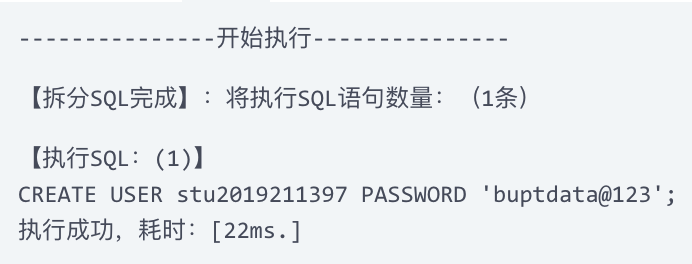
\includegraphics[width=0.5\textwidth]{./images/res1.png}
    \caption{\label{fig:res1}}
\end{figure}

\subsection{管理用户}

\subsubsection{角色管理}

选择账号管理,单击角色管理,进入角色管理页面,如\figref{fig:res2}。
\begin{figure}[!htb]
    \centering
    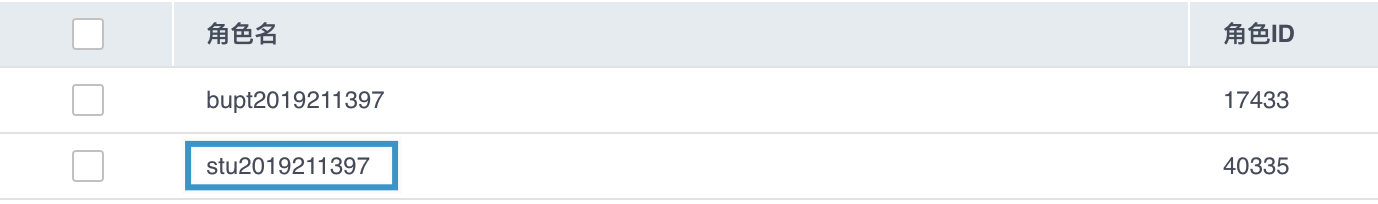
\includegraphics[width=0.8\textwidth]{./images/res2.png}
    \caption{\label{fig:res2}}
\end{figure}

单击角色名stu2019211397,进入编辑角色页面,在密码框和确认密码框输入新密码,将用户stu2019211397的登录密码由buptdata@123修改为Abcd@123,
单击保存,显示SQL预览,单击确定,修改成功,如\figref{fig:res3}。
\begin{figure}[!htb]
    \centering
    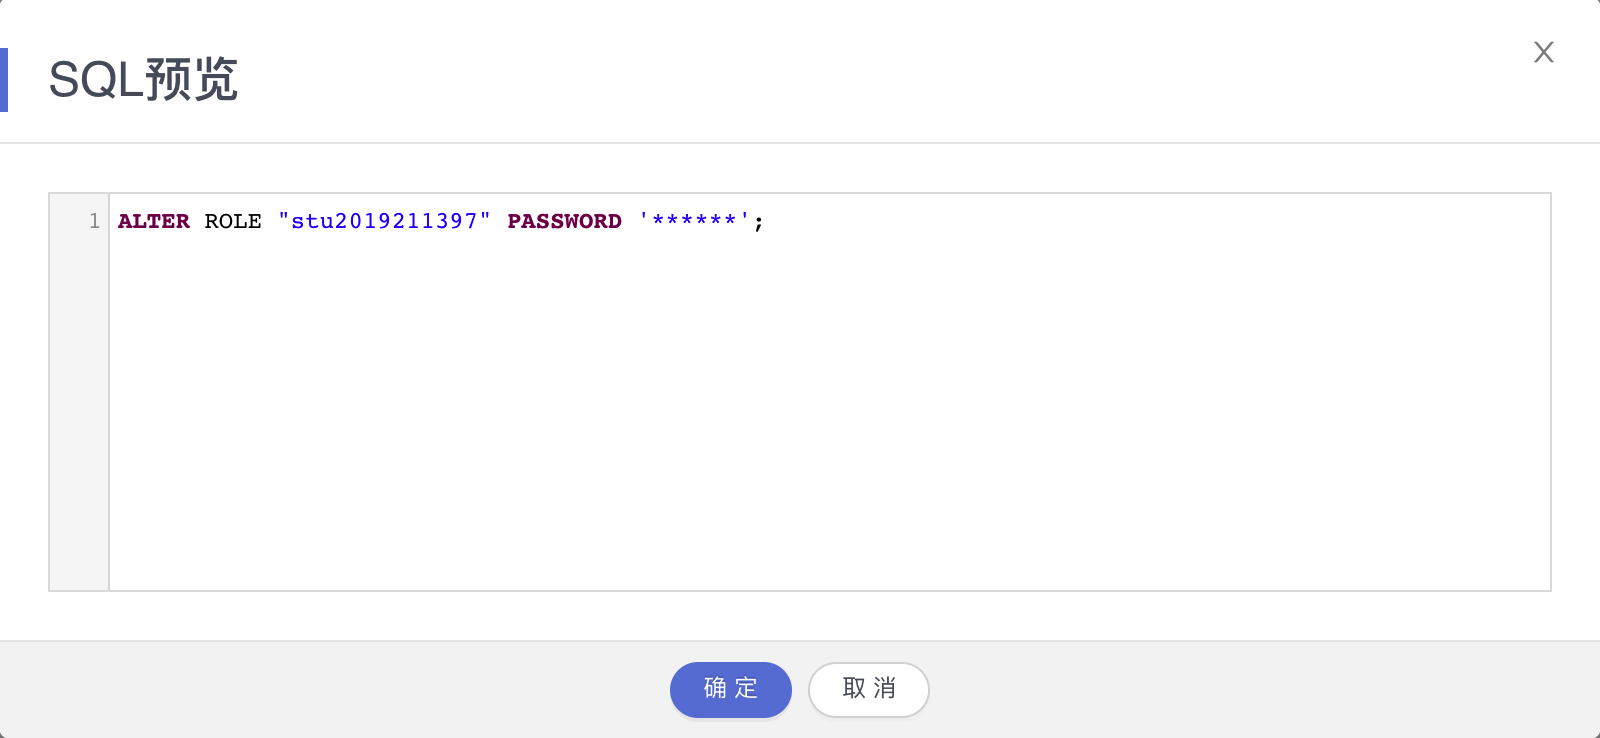
\includegraphics[width=0.7\textwidth]{./images/res3.png}
    \caption{\label{fig:res3}}
\end{figure}

为用户stu2019211397追加可以创建数据库的权限,勾选“可以创建数据库”复选框,保存,如\figref{fig:res4}。
\begin{figure}[!htb]
    \centering
    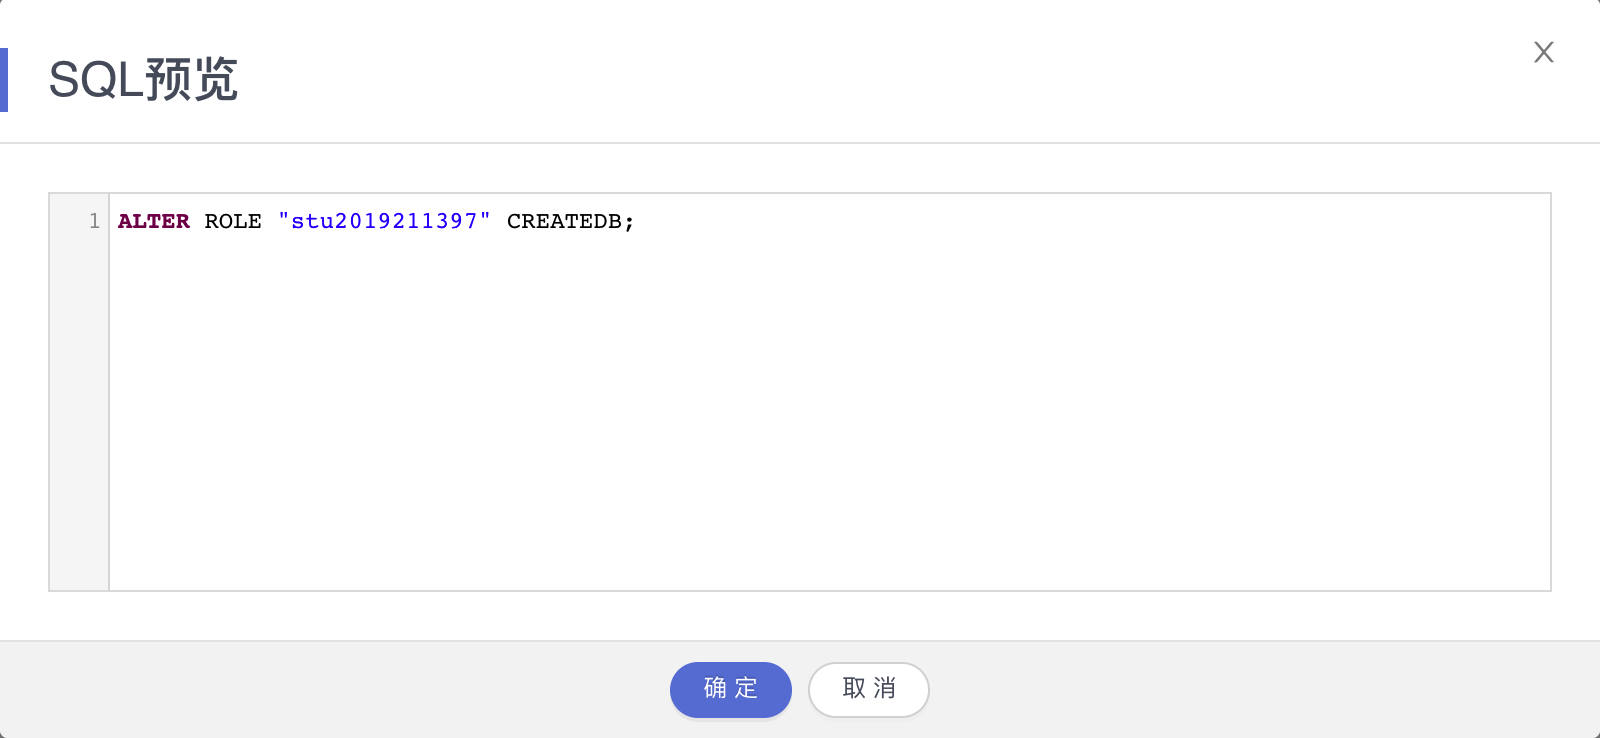
\includegraphics[width=0.7\textwidth]{./images/res4.png}
    \caption{\label{fig:res4}}
\end{figure}

将bupt2019211397角色(用户)的权限赋予stu用户,选择所属角色组,勾选bupt2019211397角色后的“授予”复选框,保存,如\figref{fig:res5}:

\begin{figure}[!htb]
    \centering
    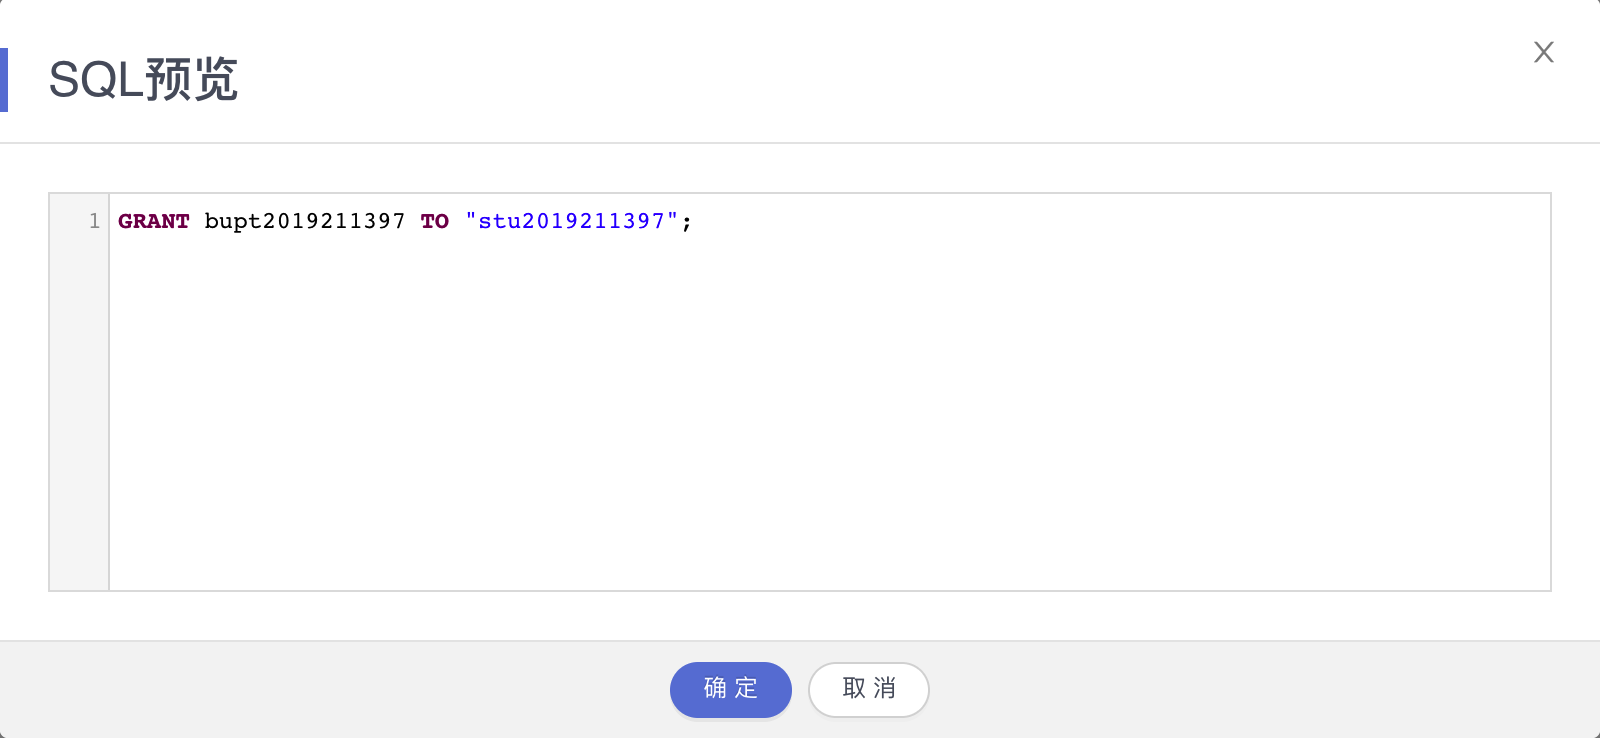
\includegraphics[width=0.7\textwidth]{./images/res5.png}
    \caption{\label{fig:res5}}
\end{figure}

\subsubsection{设置用户权限}

创建数据库yiqing\_2019211397,如\figref{fig:res6}。
\begin{figure}[!htb]
    \centering
    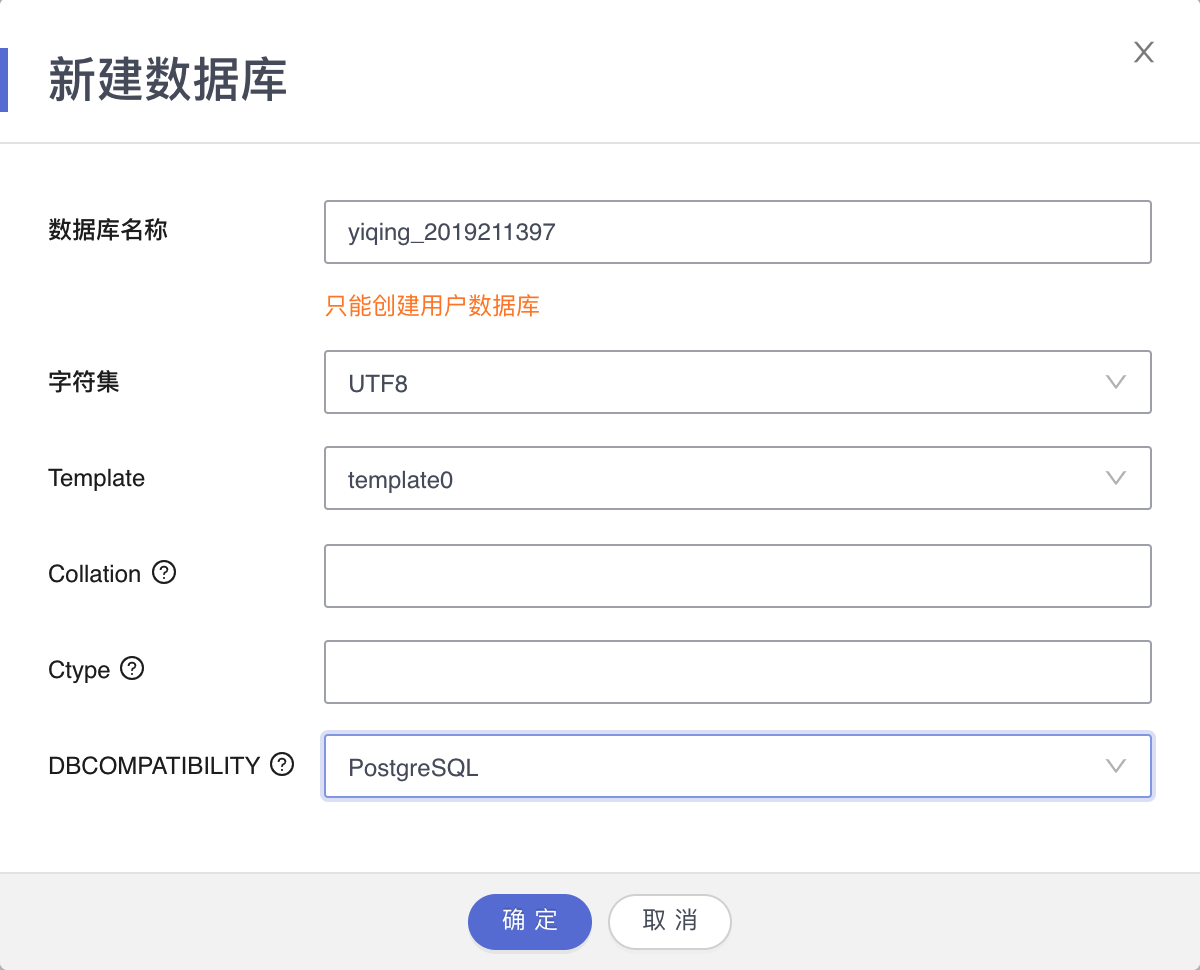
\includegraphics[width=0.6\textwidth]{./images/res6.png}
    \caption{\label{fig:res6}}
\end{figure}

创建名为root的schema,如\figref{fig:res7}。
\begin{figure}[!htb]
    \centering
    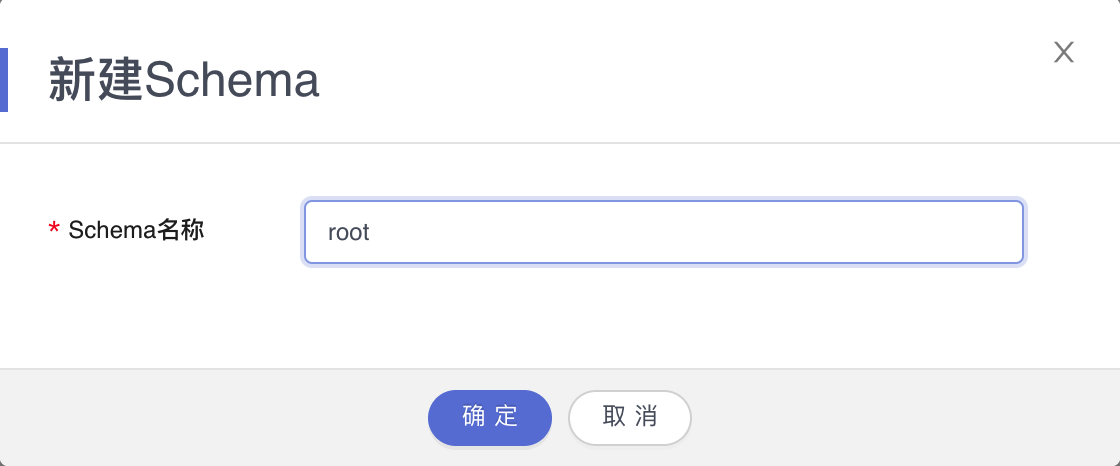
\includegraphics[width=0.6\textwidth]{./images/res7.png}
    \caption{\label{fig:res7}}
\end{figure}

单击SQL操作->SQL查询,创建一张样例表,输入以下SQL语句:
\begin{code}
\begin{minted}{sql}
CREATE TABLE 样例(testid int);
\end{minted}
\end{code}

结果如\figref{fig:res8}。
\begin{figure}[!htb]
    \centering
    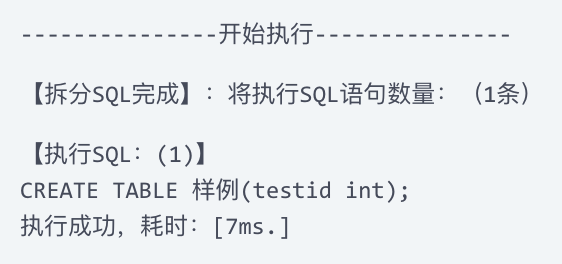
\includegraphics[width=0.5\textwidth]{./images/res8.png}
    \caption{\label{fig:res8}}
\end{figure}

单击账户管理->角色管理->单击角色名stu2019211397->权限->添加,类型选择数据库,数据库选择yiqing\_2019211397,然后单击编辑,勾选授予CONNECT权限,单击确定。

再次单击添加,类型选择Schema,数据库选择yiqing\_2019211397,Schema选择root,单击编辑,勾选授予USAGE权限,单击确定。

再次单击添加,类型选择表,数据库选择yiqing\_2019211397,Schema选择root,对象名称选择样例,单击编辑,勾选授予SELECT权限,单击确定。

如\figref{fig:res9}。
\begin{figure}[!htb]
    \centering
    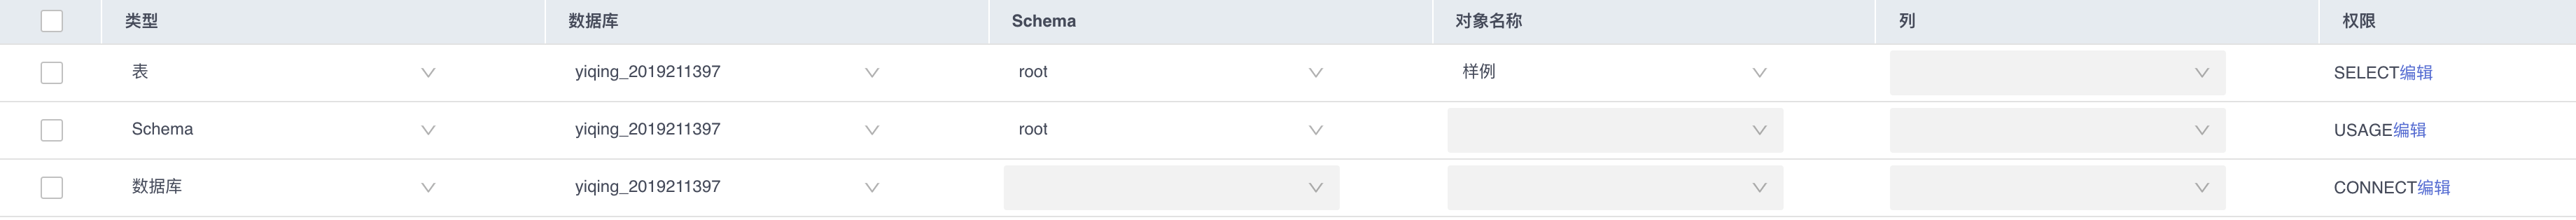
\includegraphics[width=\textwidth]{./images/res9.png}
    \caption{\label{fig:res9}}
\end{figure}

添加完成后选择保存,单击确定后,权限添加完毕,如\figref{fig:res10}。
\begin{figure}[!htb]
    \centering
    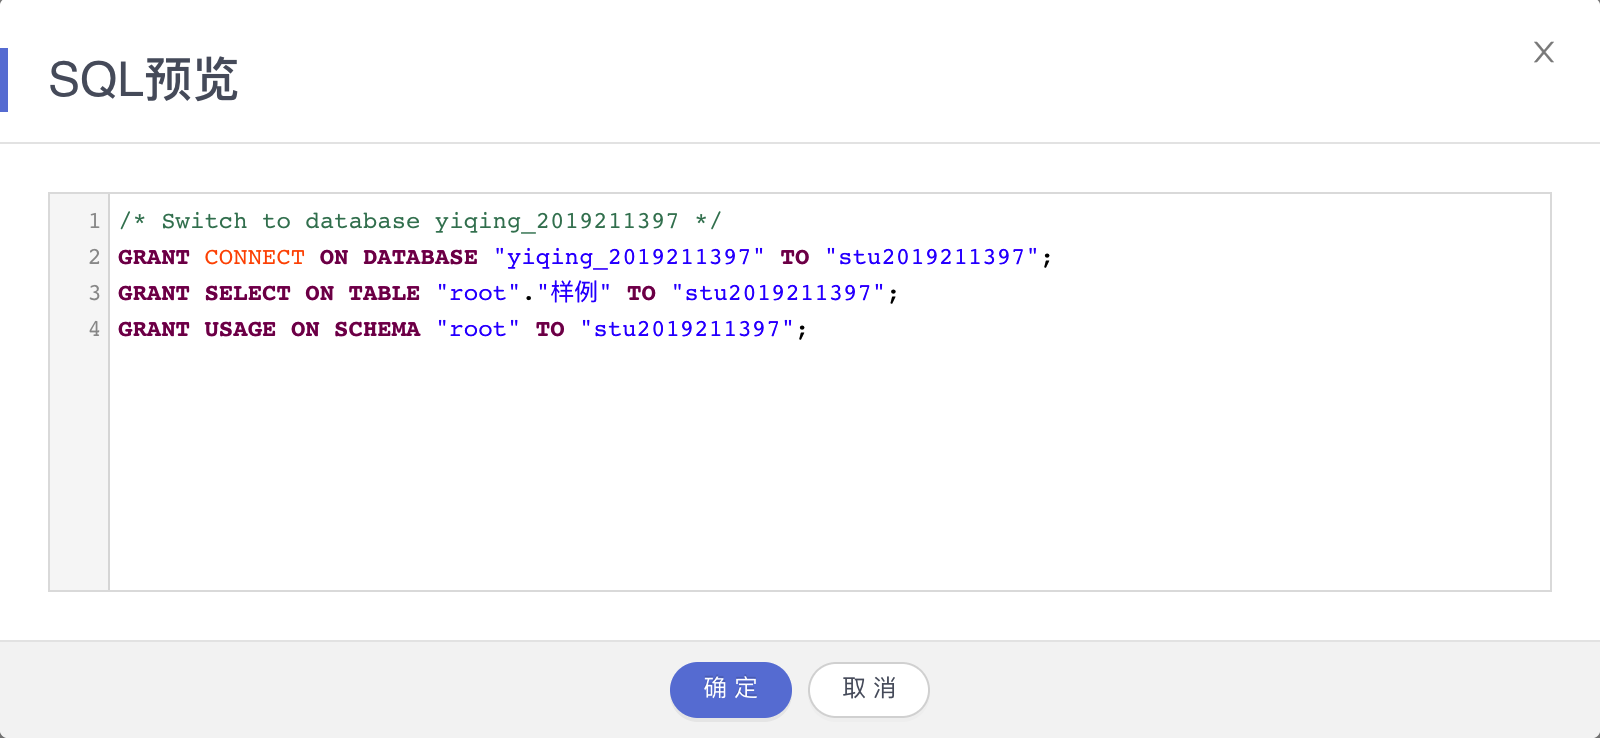
\includegraphics[width=0.7\textwidth]{./images/res10.png}
    \caption{\label{fig:res10}}
\end{figure}

\subsubsection{验证用户权限}

单击右上角账户名,选择切换连接,用stu2019211397账户登录,如\figref{fig:res11}。
\begin{figure}[!htb]
    \centering
    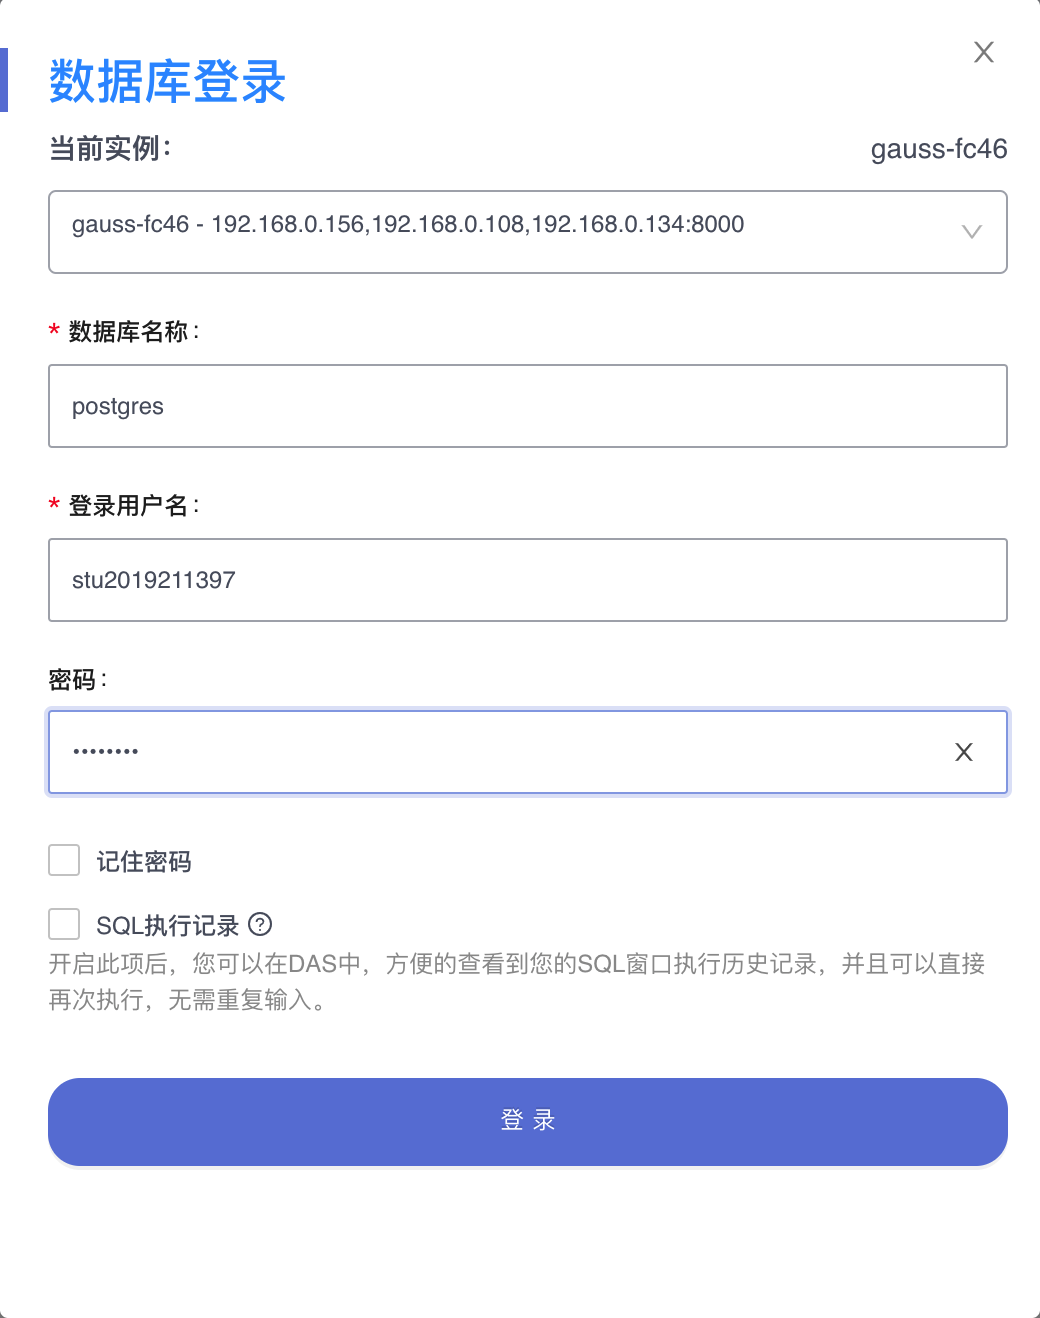
\includegraphics[width=0.5\textwidth]{./images/res11.png}
    \caption{\label{fig:res11}}
\end{figure}

进入yiqing\_2019211397数据库的SQL查询,输入以下SQL语句:
\begin{code}
\begin{minted}{sql}
SELECT * FROM 样例;
\end{minted}
\end{code}

结果如\figref{fig:res12}。
\begin{figure}[!htb]
    \centering
    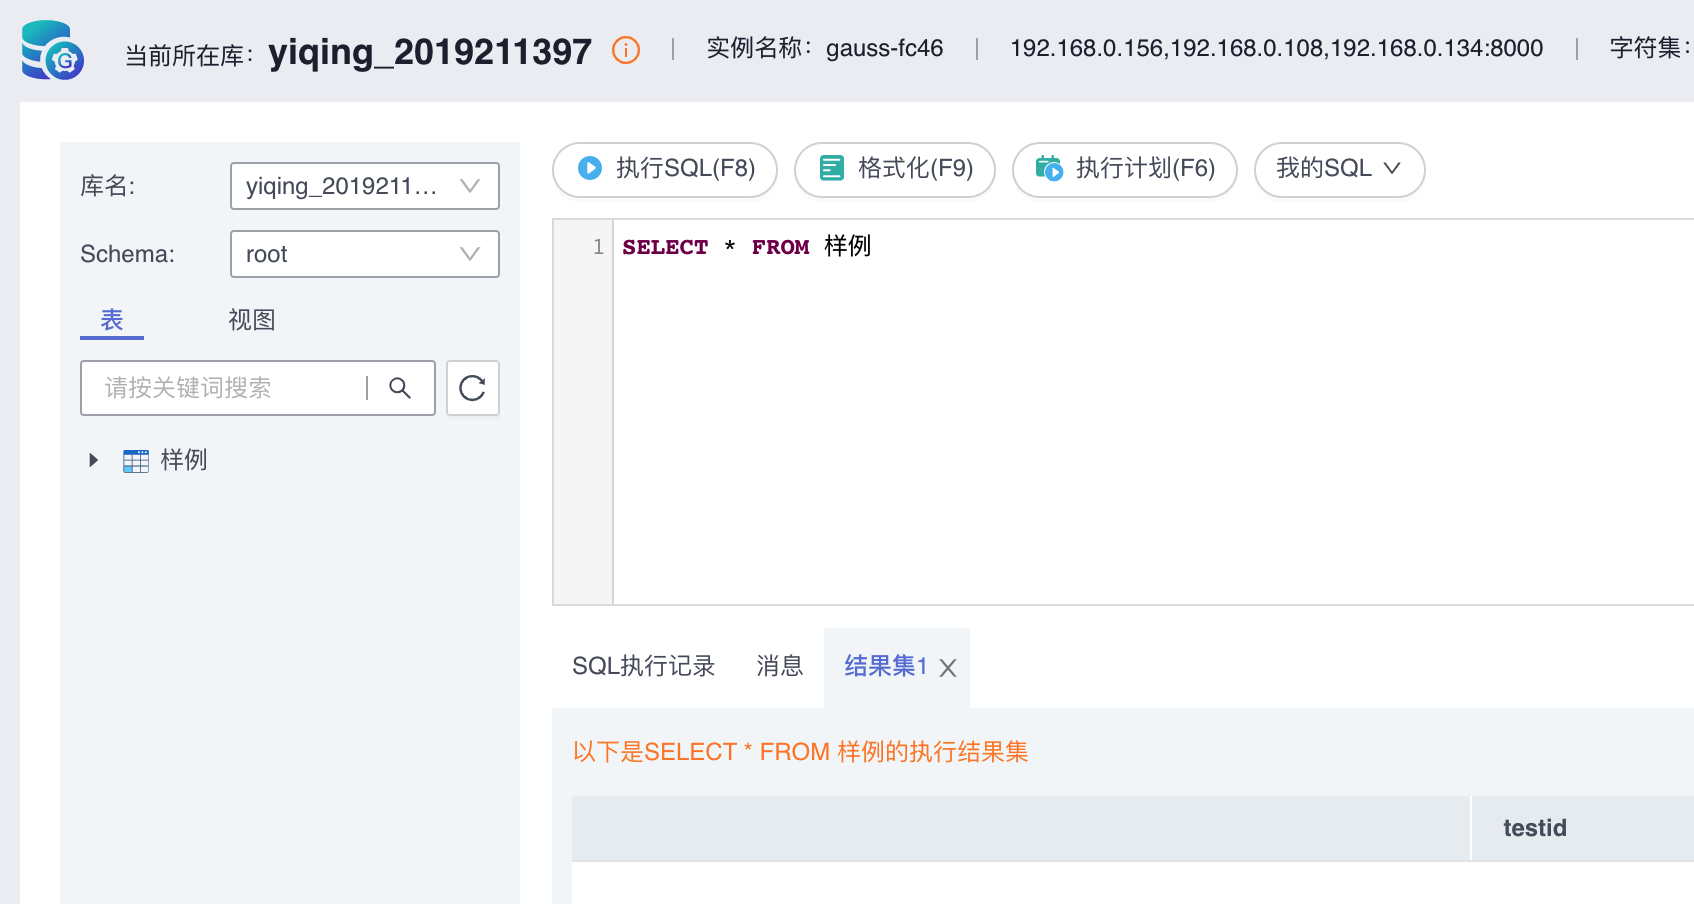
\includegraphics[width=0.7\textwidth]{./images/res12.png}
    \caption{\label{fig:res12}}
\end{figure}

\section{实验总结}

本次实验使我初步认识华为云DAS的权限管理系统,同时巩固了课堂上所学的有关用户和权限管理的知识。

\part{实验五}

\section{概述}

\subsection{实验目的}

\begin{enumerate}
    \item 通过实验让学生熟悉并了解GaussDB(for openGauss)数据库的基本机制与操作。
    \item 通过索引管理、视图管理等管理的操作,让学生熟悉并了解DAS环境下如何使用GaussDB(for openGauss)。
\end{enumerate}

\subsection{实验平台及环境}

\begin{itemize}
    \item GaussDB(for openGauss) 8 核 | 64 GB
    \item GaussDB(for openGauss) 2020主备版
\end{itemize}

\subsection{实验内容}

\begin{enumerate}
    \item 本实验通过索引管理、视图管理等管理的操作,让学生熟悉并了解DAS环境下如何使用GaussDB(for openGauss);
\end{enumerate}

\section{实验步骤}

\subsection{创建和管理索引}

\paragraph{创建索引}

进入bupt2019211397数据库,输入以下SQL语句:
\begin{code}
\begin{minted}{sql}
CREATE INDEX 日期index ON 美国各州县确诊与死亡数统计表(日期);
\end{minted}
\end{code}

结果如\figref{fig:res13}。
\begin{figure}[!htb]
    \centering
    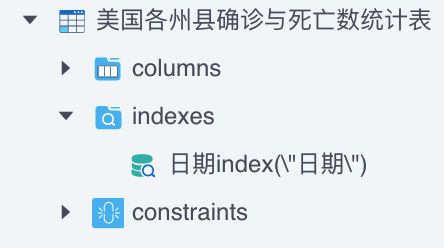
\includegraphics[width=0.4\textwidth]{./images/res13.png}
    \caption{\label{fig:res13}}
\end{figure}

\paragraph{管理索引}

创建索引后刷新页面,左下角会显示表视图,单击indexes显示当前表的所有索引,如\figref{fig:res13}。

删除索引,输入以下SQL语句:
\begin{code}
\begin{minted}{sql}
DROP INDEX 日期index;
\end{minted}
\end{code}

\paragraph{索引创建练习}

创建唯一索引,输入以下SQL语句:
\begin{code}
\begin{minted}{sql}
CREATE INDEX 日期index ON 美国各州县确诊与死亡数统计表(日期);
\end{minted}
\end{code}

输入以下SQL语句进行查询:
\begin{code}
\begin{minted}{sql}
SELECT 日期 FROM 美国各州县确诊与死亡数统计表 WHERE 日期='2020-12-24';
\end{minted}
\end{code}

创建索引前和索引后的结果分别如\figref{fig:res14}和\figref{fig:res15}。
\begin{figure}[!htb]
    \centering
    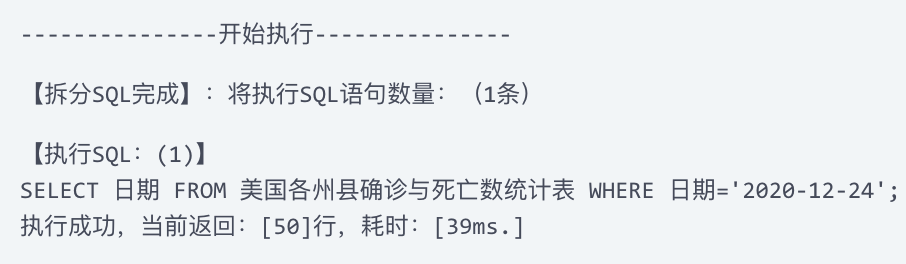
\includegraphics[width=0.5\textwidth]{./images/res14.png}
    \caption{\label{fig:res14}}
\end{figure}
\begin{figure}[!htb]
    \centering
    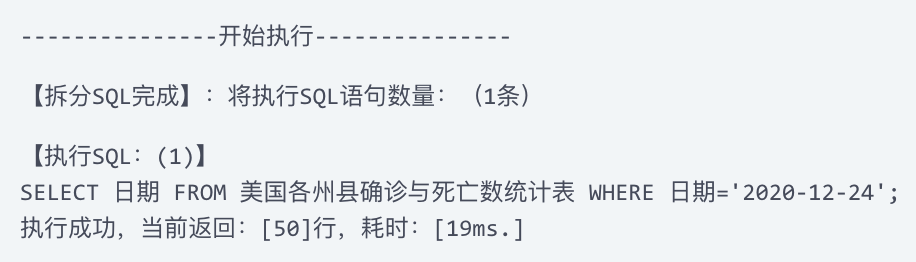
\includegraphics[width=0.5\textwidth]{./images/res15.png}
    \caption{\label{fig:res15}}
\end{figure}

可见查询效率有提升。

创建多字段索引,输入以下SQL语句:
\begin{code}
\begin{minted}{sql}
CREATE INDEX 累计index ON 美国各州县确诊与死亡数统计表(日期,累计确诊);
\end{minted}
\end{code}

输入以下SQL语句进行查询:
\begin{code}
\begin{minted}{sql}
SELECT * FROM 美国各州县确诊与死亡数统计表 WHERE 日期='2020-12-24' AND 累计确诊>1000;
\end{minted}
\end{code}

创建索引前和索引后的结果分别如\figref{fig:res16}和\figref{fig:res17}。
\begin{figure}[!htb]
    \centering
    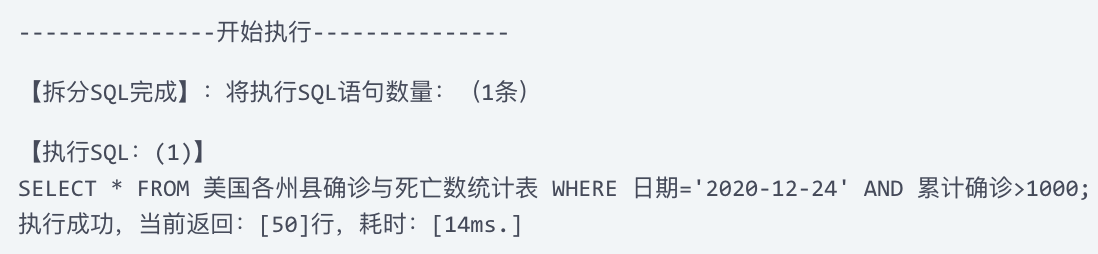
\includegraphics[width=0.5\textwidth]{./images/res16.png}
    \caption{\label{fig:res16}}
\end{figure}
\begin{figure}[!htb]
    \centering
    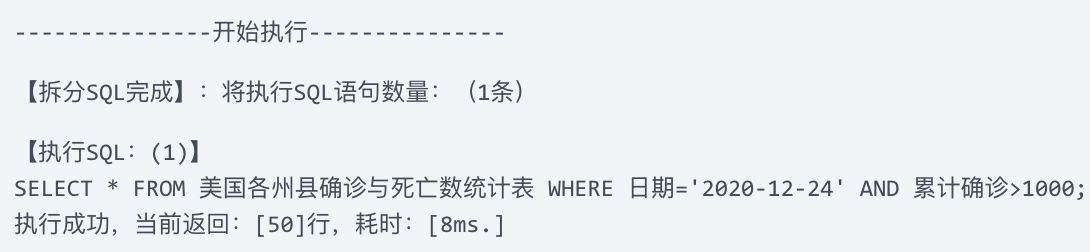
\includegraphics[width=0.5\textwidth]{./images/res17.png}
    \caption{\label{fig:res17}}
\end{figure}

可见查询效率有提升。

如果只需要查询日期='2020-12-24'的记录,可以创建部分索引来提升查询效率,输入以下SQL语句:
\begin{code}
\begin{minted}{sql}
CREATE INDEX 日期index ON 美国各州县确诊与死亡数统计表(日期) WHERE 日期 = '2020-12-24';
\end{minted}
\end{code}

输入以下SQL语句进行查询:
\begin{code}
\begin{minted}{sql}
SELECT 日期 FROM 美国各州县确诊与死亡数统计表 WHERE 日期='2020-12-24';
\end{minted}
\end{code}

创建索引前和索引后的结果分别如\figref{fig:res14}和\figref{fig:res18}。
\begin{figure}[!htb]
    \centering
    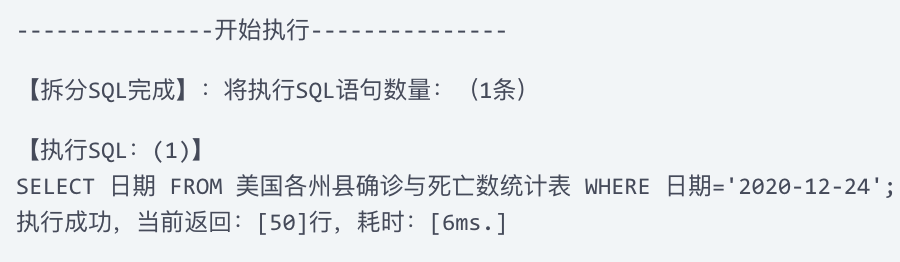
\includegraphics[width=0.5\textwidth]{./images/res18.png}
    \caption{\label{fig:res18}}
\end{figure}

可见查询效率有提升。

创建表达式索引,输入以下SQL语句:
\begin{code}
\begin{minted}{sql}
CREATE INDEX 累计确诊index ON 美国各州县确诊与死亡数统计表(trunc(累计确诊));
\end{minted}
\end{code}

输入以下SQL语句进行查询:
\begin{code}
\begin{minted}{sql}
SELECT * FROM 美国各州县确诊与死亡数统计表 WHERE trunc(累计确诊)>1000;
\end{minted}
\end{code}

创建索引前和索引后的结果分别如\figref{fig:res19}和\figref{fig:res20}。
\begin{figure}[!htb]
    \centering
    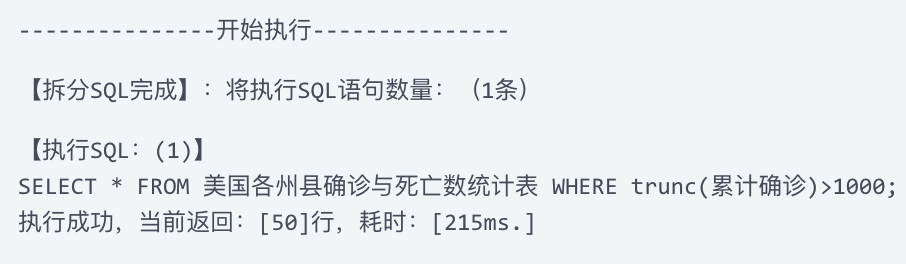
\includegraphics[width=0.5\textwidth]{./images/res19.png}
    \caption{\label{fig:res19}}
\end{figure}
\begin{figure}[!htb]
    \centering
    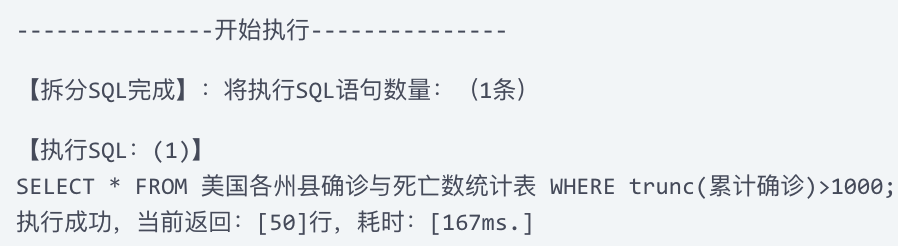
\includegraphics[width=0.5\textwidth]{./images/res20.png}
    \caption{\label{fig:res20}}
\end{figure}

可见查询效率有提升。

\subsection{创建和管理视图}

创建普通视图bj\_yq,输入以下SQL语句:
\begin{code}
\begin{minted}{sql}
CREATE VIEW bj_yq AS
SELECT 行程号, x.病例号, 性别, x.日期信息, 行程信息
FROM 病例行程信息表 x LEFT JOIN 病例基本信息表 y
ON x.病例号 = y.病例号
WHERE y.省 = '北京市';
\end{minted}
\end{code}

进入对象列表,单击视图,如\figref{fig:res21}。
\begin{figure}[!htb]
    \centering
    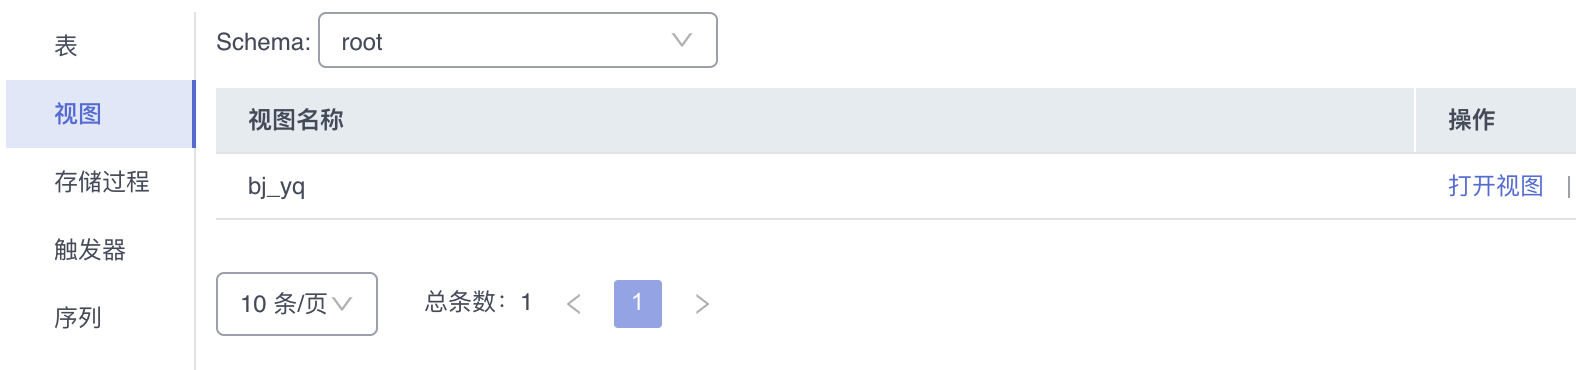
\includegraphics[width=0.7\textwidth]{./images/res21.png}
    \caption{\label{fig:res21}}
\end{figure}

查询视图bj\_yq,输入以下SQL语句:
\begin{code}
\begin{minted}{sql}
SELECT * FROM bj_yq;
\end{minted}
\end{code}

结果如\figref{fig:res22}。
\begin{figure}[!htb]
    \centering
    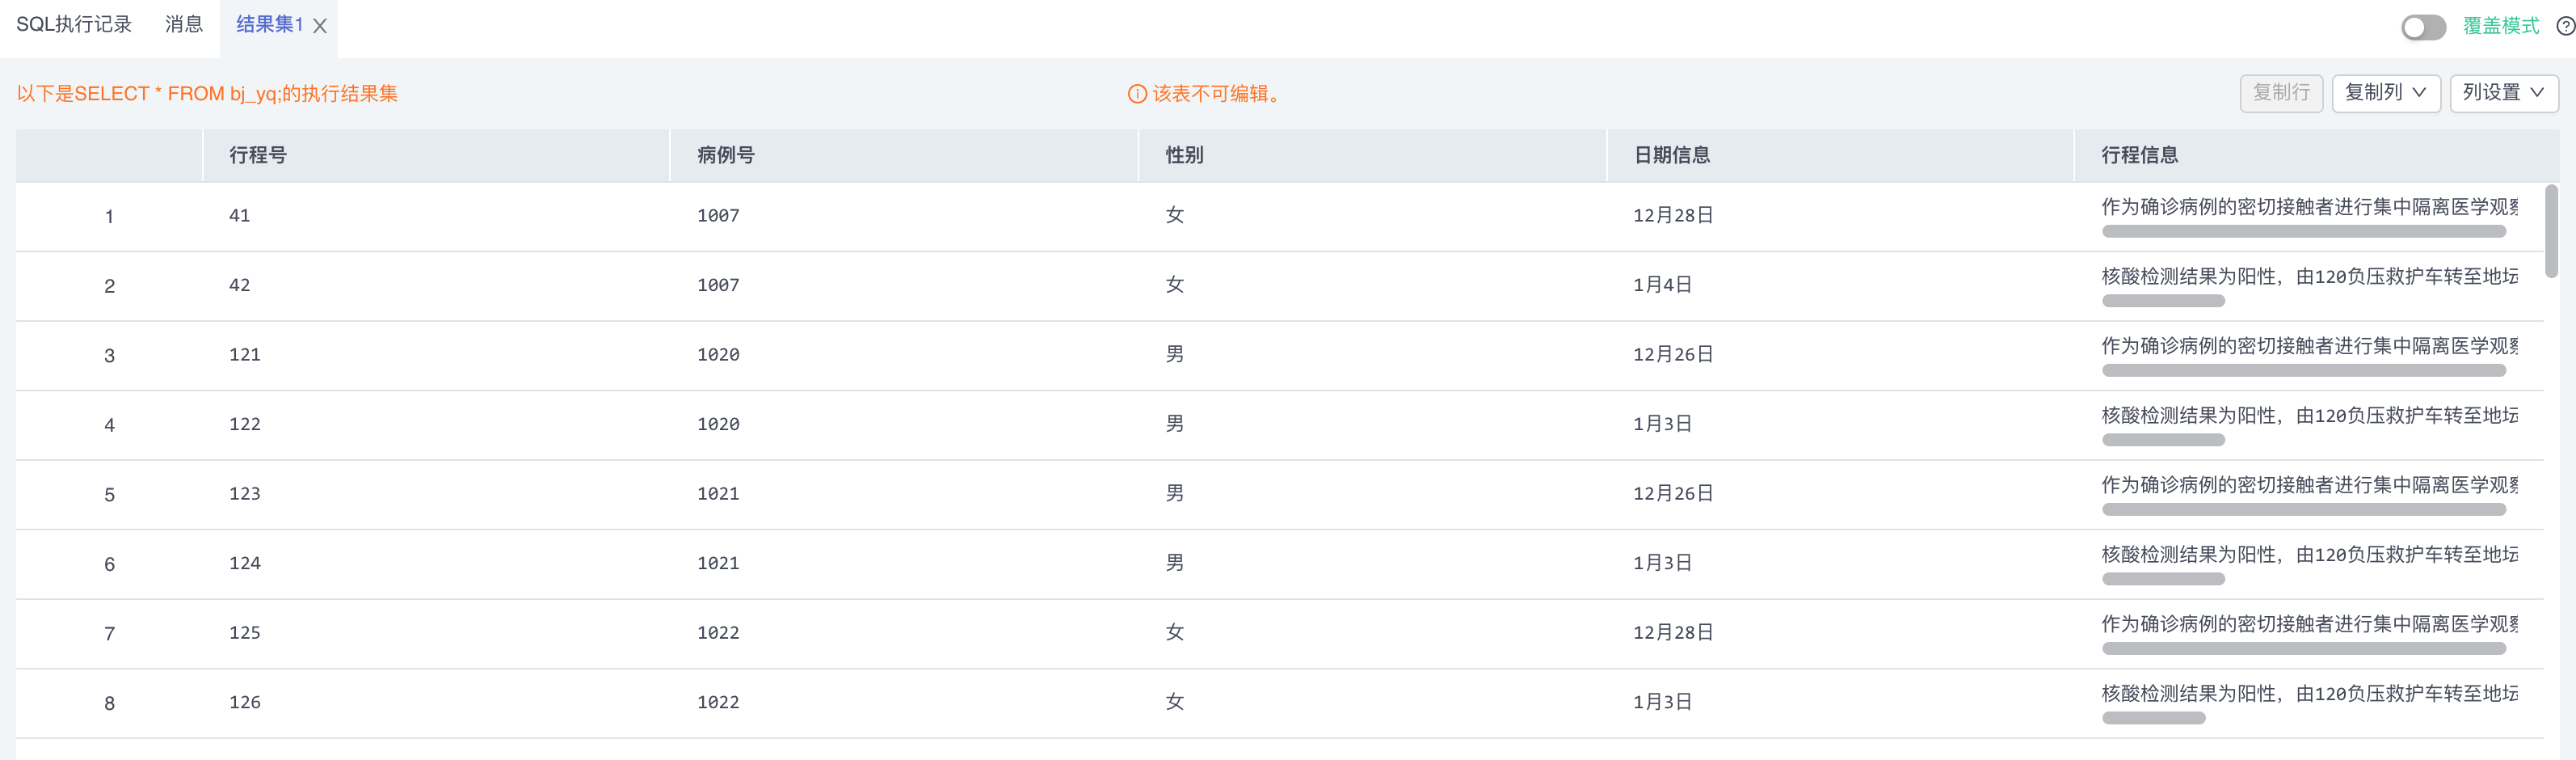
\includegraphics[width=\textwidth]{./images/res22.png}
    \caption{\label{fig:res22}}
\end{figure}

进入对象列表,单击视图,单击查看视图详情,如\figref{fig:res23}。
\begin{figure}[!htb]
    \centering
    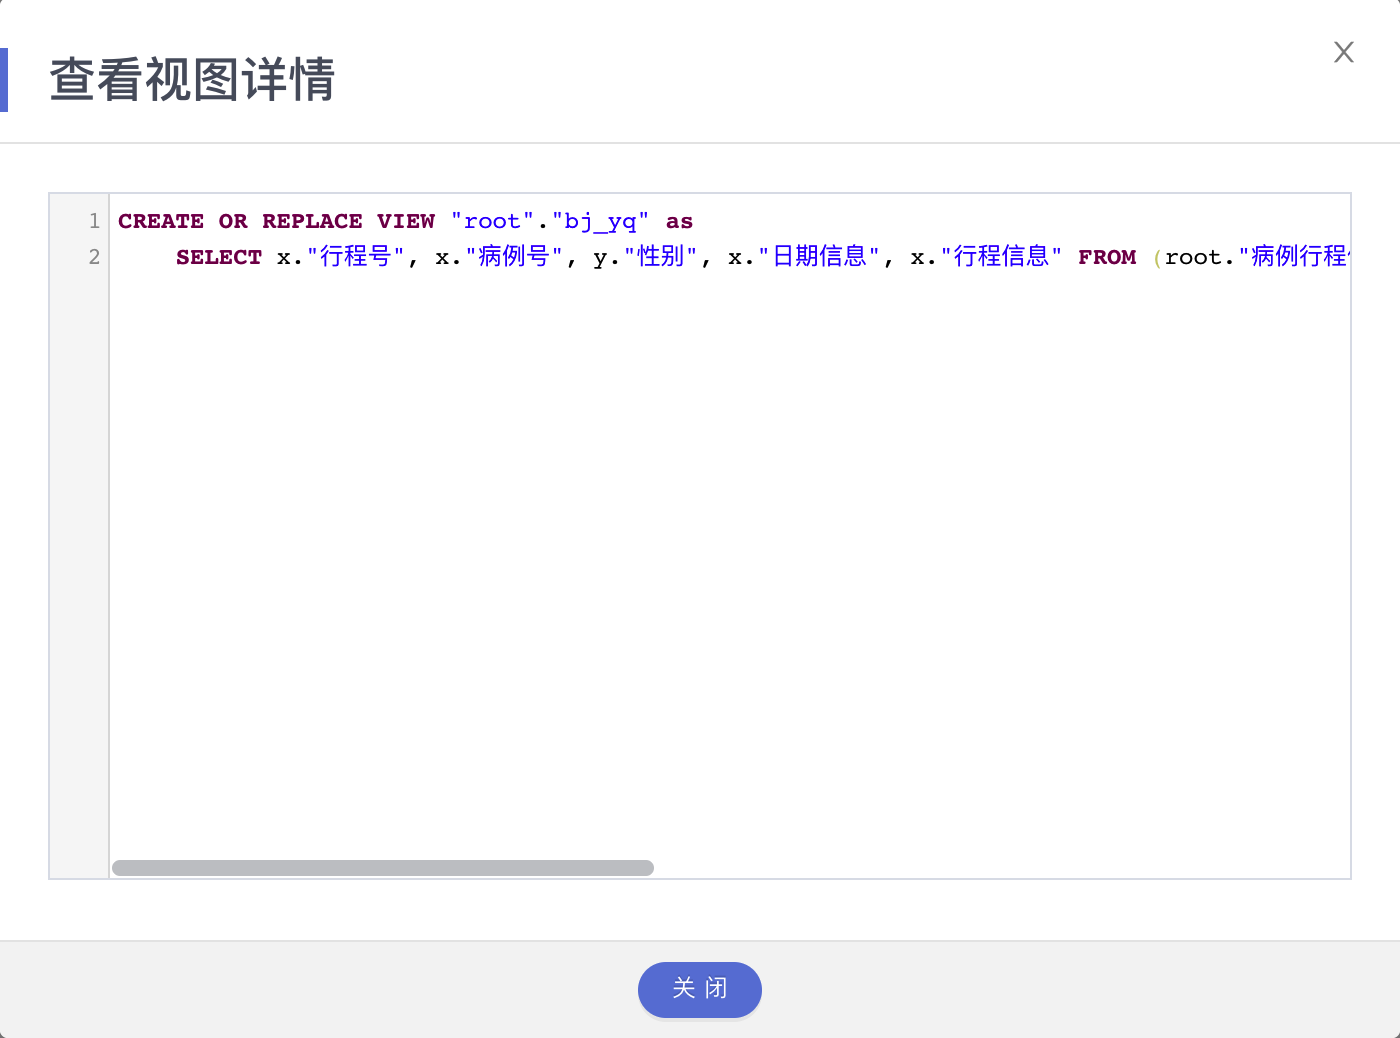
\includegraphics[width=0.7\textwidth]{./images/res23.png}
    \caption{\label{fig:res23}}
\end{figure}

查询临床分型为普通型的病例号、行程号、性别和日期信息,按照病例号进行升序显示(截前五条记录),输入以下SQL语句:
\begin{code}
\begin{minted}{sql}
SELECT 病例号, 行程号, 性别, 日期信息
FROM bj_yq
WHERE 行程信息 LIKE '%普通型%'
ORDER BY 病例号;
\end{minted}
\end{code}

结果如\figref{fig:res24}。
\begin{figure}[!htb]
    \centering
    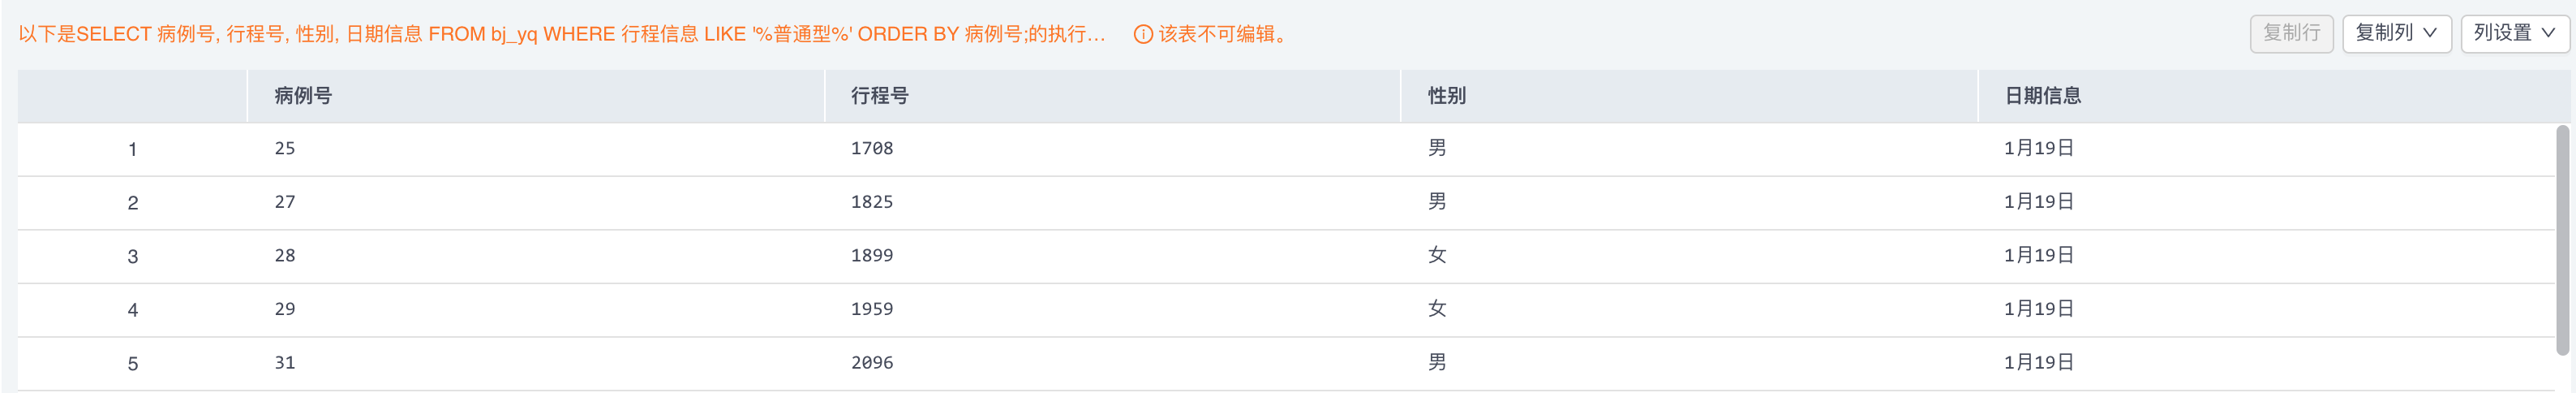
\includegraphics[width=\textwidth]{./images/res24.png}
    \caption{\label{fig:res24}}
\end{figure}

\section{实验总结}

本次实验使我对SQL的索引和视图有关语法更加熟悉,并且了解了几种不同类型的索引,同时巩固了课堂上所学的索引和视图的知识。

\part{实验六}

\section{概述}

\subsection{实验目的}

\begin{enumerate}
    \item 通过实验让学生熟悉并了解GaussDB(for openGauss)数据库的基本机制与操作。
    \item 通过创建和管理存储过程、触发器等操作,让学生熟悉并了解DAS环境下如何使用GaussDB(for openGauss)。
\end{enumerate}

\subsection{实验平台及环境}

\begin{itemize}
    \item GaussDB(for openGauss) 8 核 | 64 GB
    \item GaussDB(for openGauss) 2020主备版
\end{itemize}

\subsection{实验内容}

\begin{enumerate}
    \item 本实验通过存储过程管理、触发器管理等操作,让学生熟悉并了解DAS环境下如何使用GaussDB(for openGauss);
\end{enumerate}

\section{实验步骤}

\subsection{创建存储过程}

在全国各省累计数据统计表中增加一条记录。执行存储过程:增加2021年10月8日吉林省累计确诊578例,累计治愈571例,累计死亡3例。

创建存储过程insertRecord,内容如\figref{fig:res25}。
\begin{figure}[!htb]
    \centering
    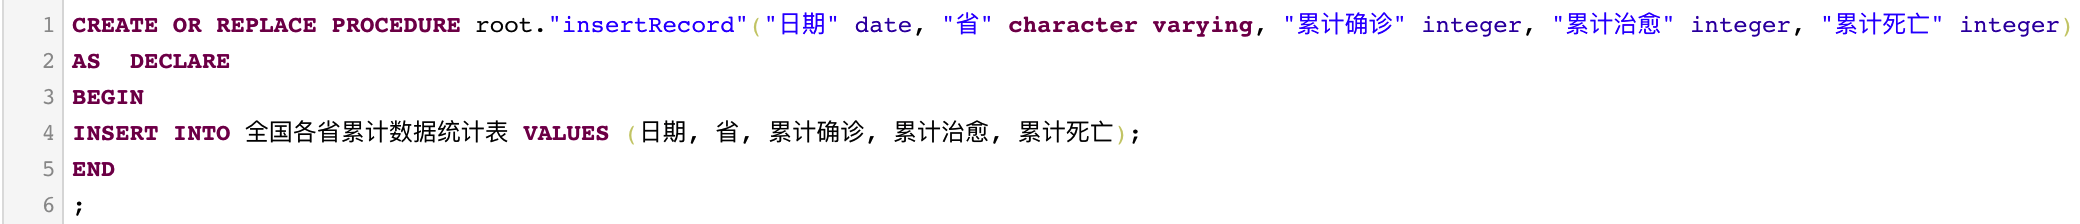
\includegraphics[width=\textwidth]{./images/res25.png}
    \caption{\label{fig:res25}}
\end{figure}

执行存储过程,设置参数如\figref{fig:res26}。
\begin{figure}[!htb]
    \centering
    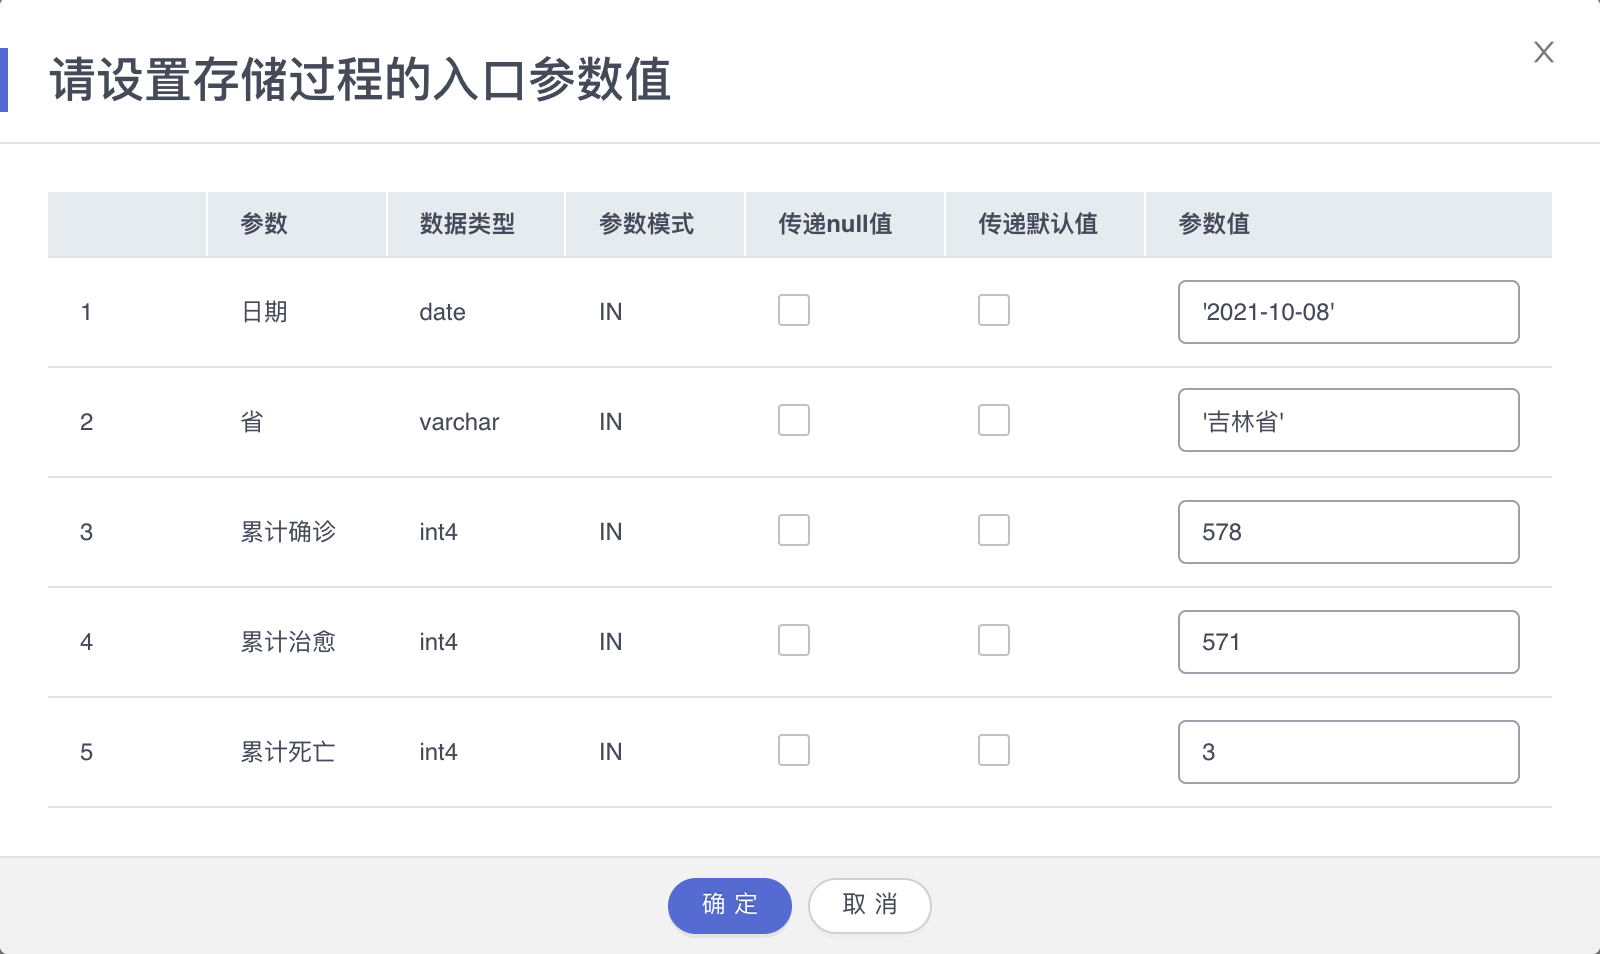
\includegraphics[width=0.7\textwidth]{./images/res26.png}
    \caption{\label{fig:res26}}
\end{figure}

执行结果如\figref{fig:res27}。
\begin{figure}[!htb]
    \centering
    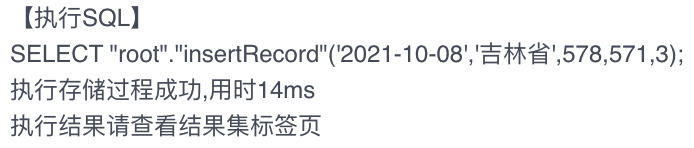
\includegraphics[width=0.5\textwidth]{./images/res27.png}
    \caption{\label{fig:res27}}
\end{figure}

查询美国指定州指定日期的新冠肺炎累计确诊总数与累计死亡总数。通过该存储过程统计California州截至2021年1月1日的新冠疫情数据情况。

创建存储过程queryRecord,内容如\figref{fig:res28}。
\begin{figure}[!htb]
    \centering
    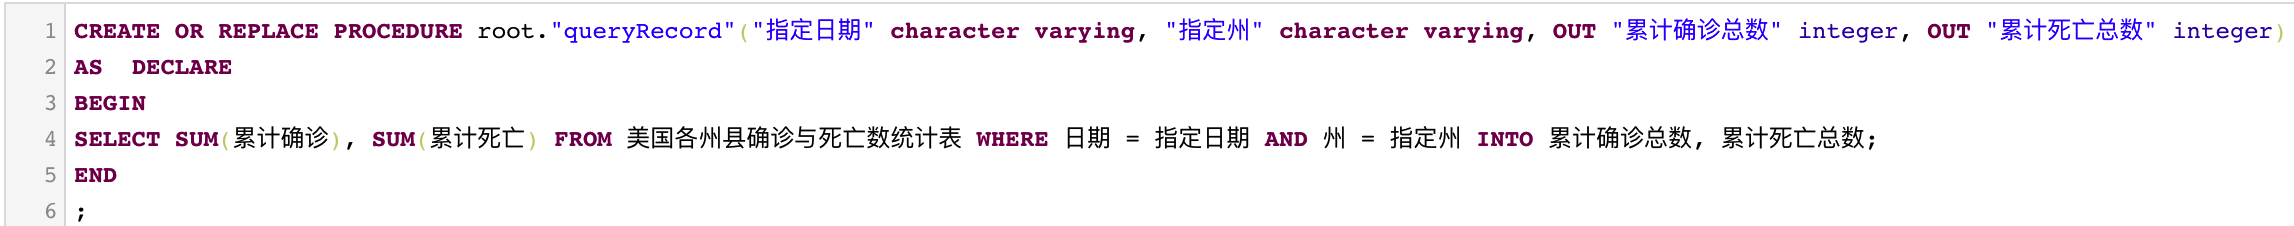
\includegraphics[width=\textwidth]{./images/res28.png}
    \caption{\label{fig:res28}}
\end{figure}

执行存储过程,设置参数如\figref{fig:res29}。
\begin{figure}[!htb]
    \centering
    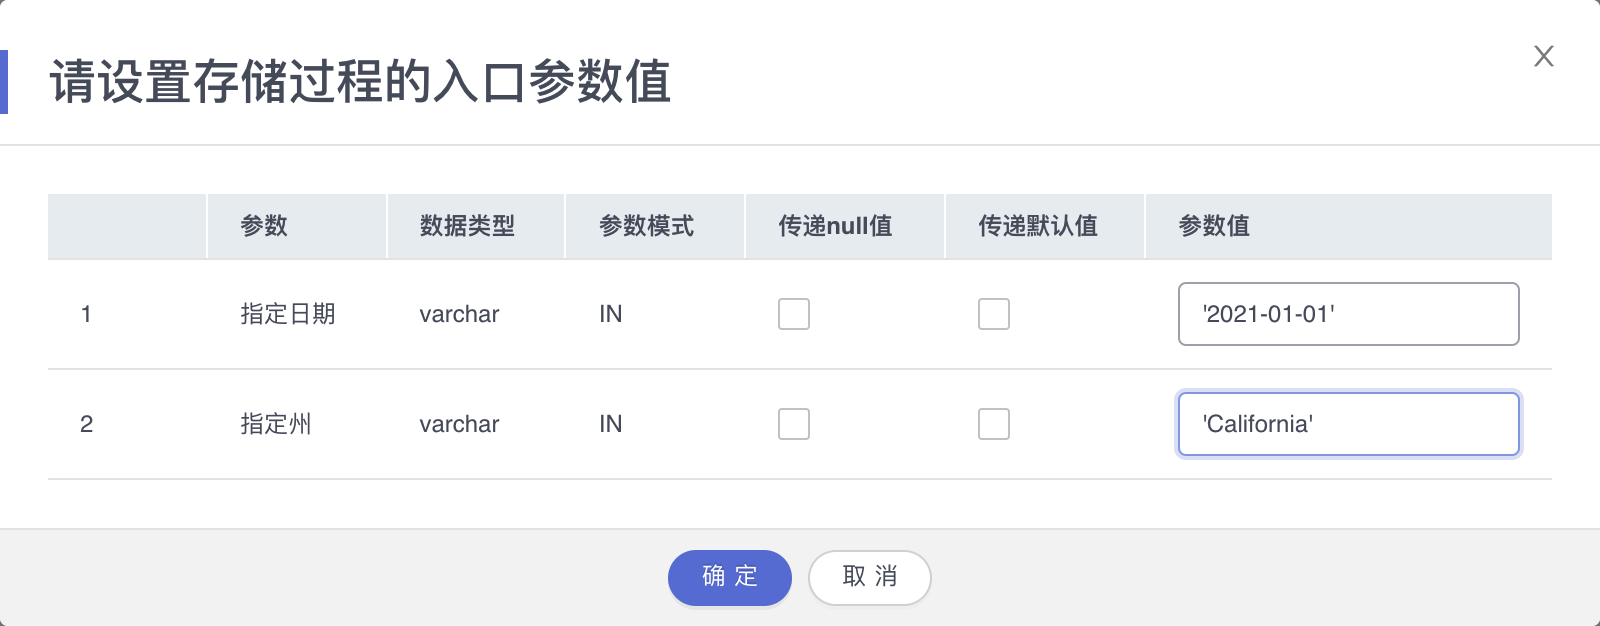
\includegraphics[width=0.7\textwidth]{./images/res29.png}
    \caption{\label{fig:res29}}
\end{figure}

执行结果如\figref{fig:res30}。
\begin{figure}[!htb]
    \centering
    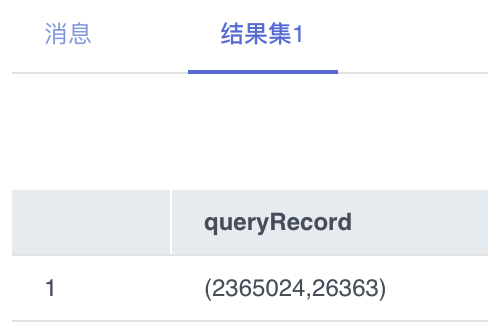
\includegraphics[width=0.3\textwidth]{./images/res30.png}
    \caption{\label{fig:res30}}
\end{figure}

\subsection{管理存储过程}

管理存储过程,切换到库管理->对象列表,选择存储过程,选择insertRecord存储过程中的操作,单击查看存储过程详情,如\figref{fig:res31}。
\begin{figure}[!htb]
    \centering
    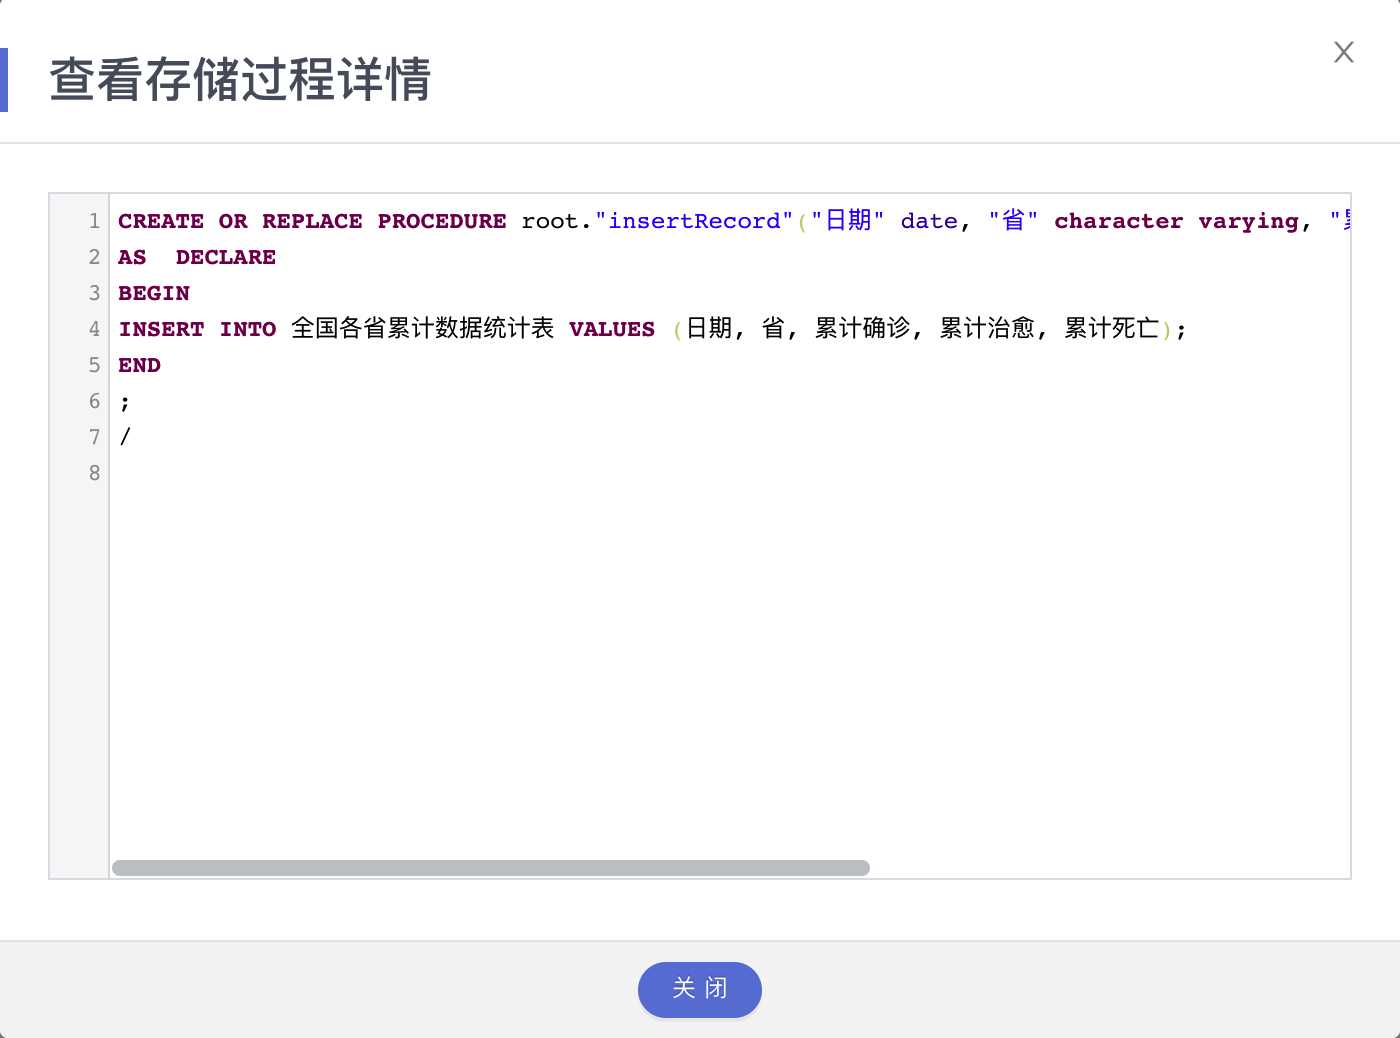
\includegraphics[width=0.7\textwidth]{./images/res31.png}
    \caption{\label{fig:res31}}
\end{figure}

删除存储过程,输入以下SQL语句:
\begin{code}
\begin{minted}{sql}
drop procedure "insertRecord";
\end{minted}
\end{code}

结果如\figref{fig:res32}。
\begin{figure}[!htb]
    \centering
    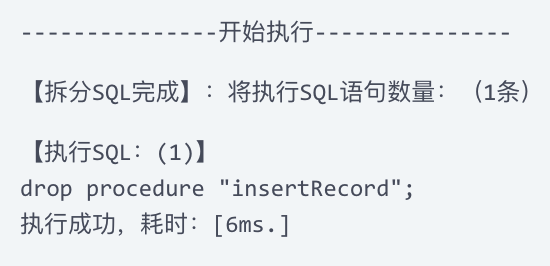
\includegraphics[width=0.4\textwidth]{./images/res32.png}
    \caption{\label{fig:res32}}
\end{figure}

\subsection{创建触发器}

创建INSERT触发器,向美国各州县确诊与死亡数统计表中插入记录时,检查该记录的州县在参考信息表中是否存在。如果不存在,则不允许插入。

创建函数check\_on\_insert,如\figref{fig:res33}。
\begin{figure}[!htb]
    \centering
    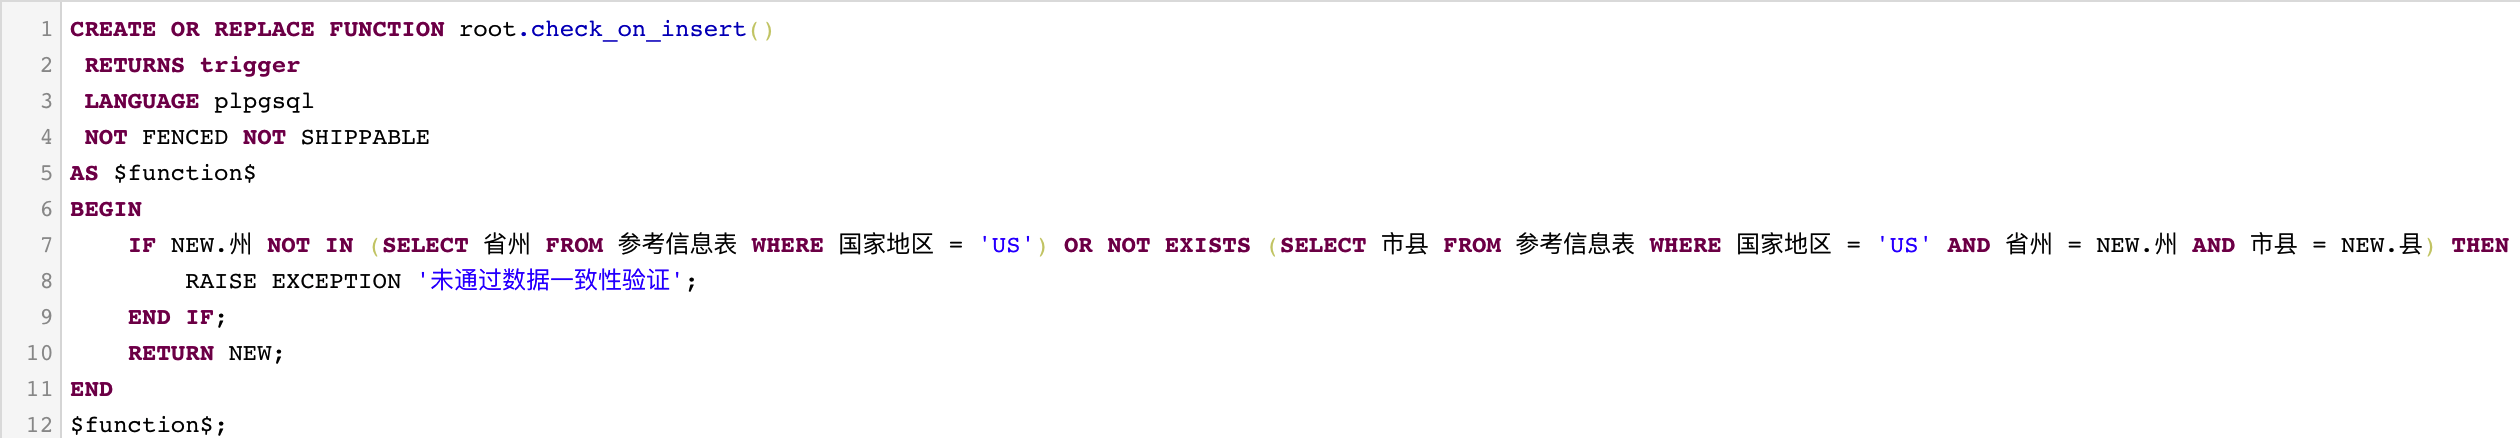
\includegraphics[width=\textwidth]{./images/res33.png}
    \caption{\label{fig:res33}}
\end{figure}

创建触发器,输入以下SQL语句:
\begin{code}
\begin{minted}{sql}
CREATE TRIGGER trigger_insert BEFORE INSERT ON 美国各州县确诊与死亡数统计表 FOR EACH ROW EXECUTE PROCEDURE check_on_insert();
\end{minted}
\end{code}

输入以下SQL语句测试:
\begin{code}
\begin{minted}{sql}
INSERT INTO 美国各州县确诊与死亡数统计表 VALUES ('2021-10-19', 'US', 'AAA', 'BBB', 123, 1);
\end{minted}
\end{code}

结果如\figref{fig:res34}。
\begin{figure}[!htb]
    \centering
    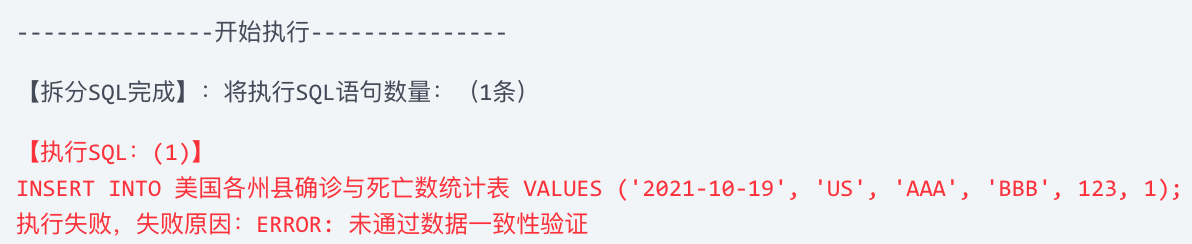
\includegraphics[width=0.6\textwidth]{./images/res34.png}
    \caption{\label{fig:res34}}
\end{figure}

创建DELETE触发器,当从病例基本信息表中删除一条记录时,该病例ID对应的行程信息记录也进行删除操作。

创建函数on\_delete,如\figref{fig:res35}。
\begin{figure}[!htb]
    \centering
    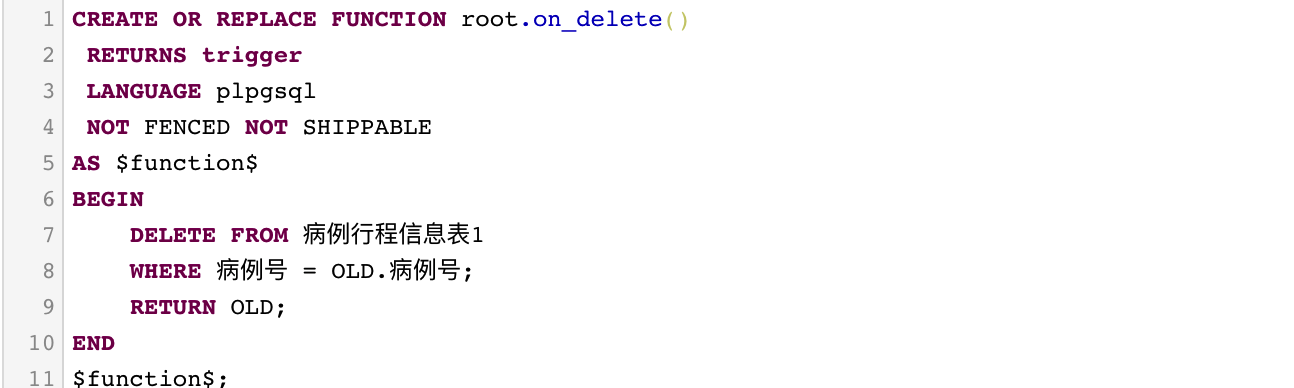
\includegraphics[width=\textwidth]{./images/res35.png}
    \caption{\label{fig:res35}}
\end{figure}

创建触发器,输入以下SQL语句:
\begin{code}
\begin{minted}{sql}
CREATE TRIGGER trigger_delete AFTER DELETE ON 病例基本信息表1 FOR EACH ROW EXECUTE PROCEDURE on_delete();
\end{minted}
\end{code}

查看病例基本信息表和病例行程信息表中病例号为1的患者的信息,如\figref{fig:res36}和\figref{fig:res37}。
\begin{figure}[!htb]
    \centering
    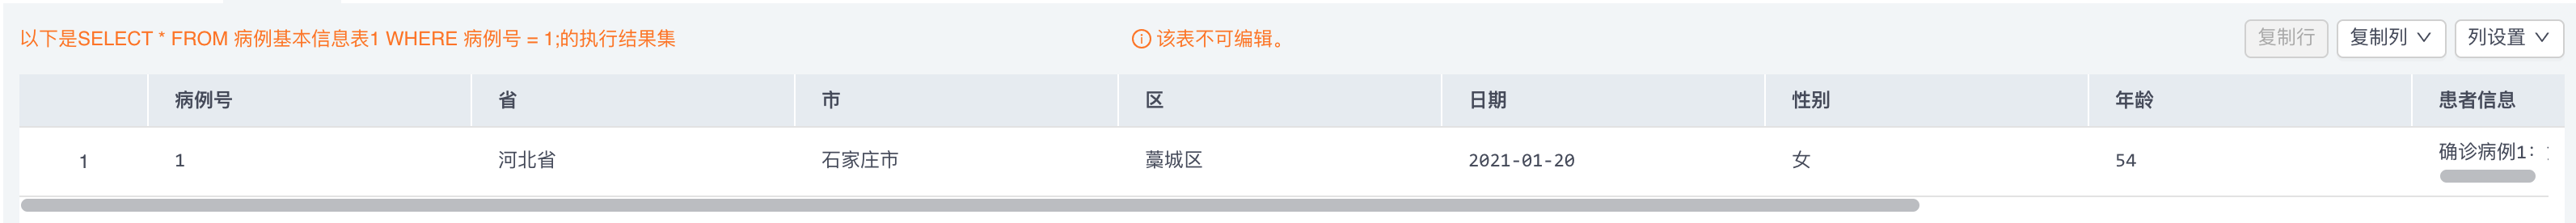
\includegraphics[width=\textwidth]{./images/res36.png}
    \caption{\label{fig:res36}}
\end{figure}
\begin{figure}[!htb]
    \centering
    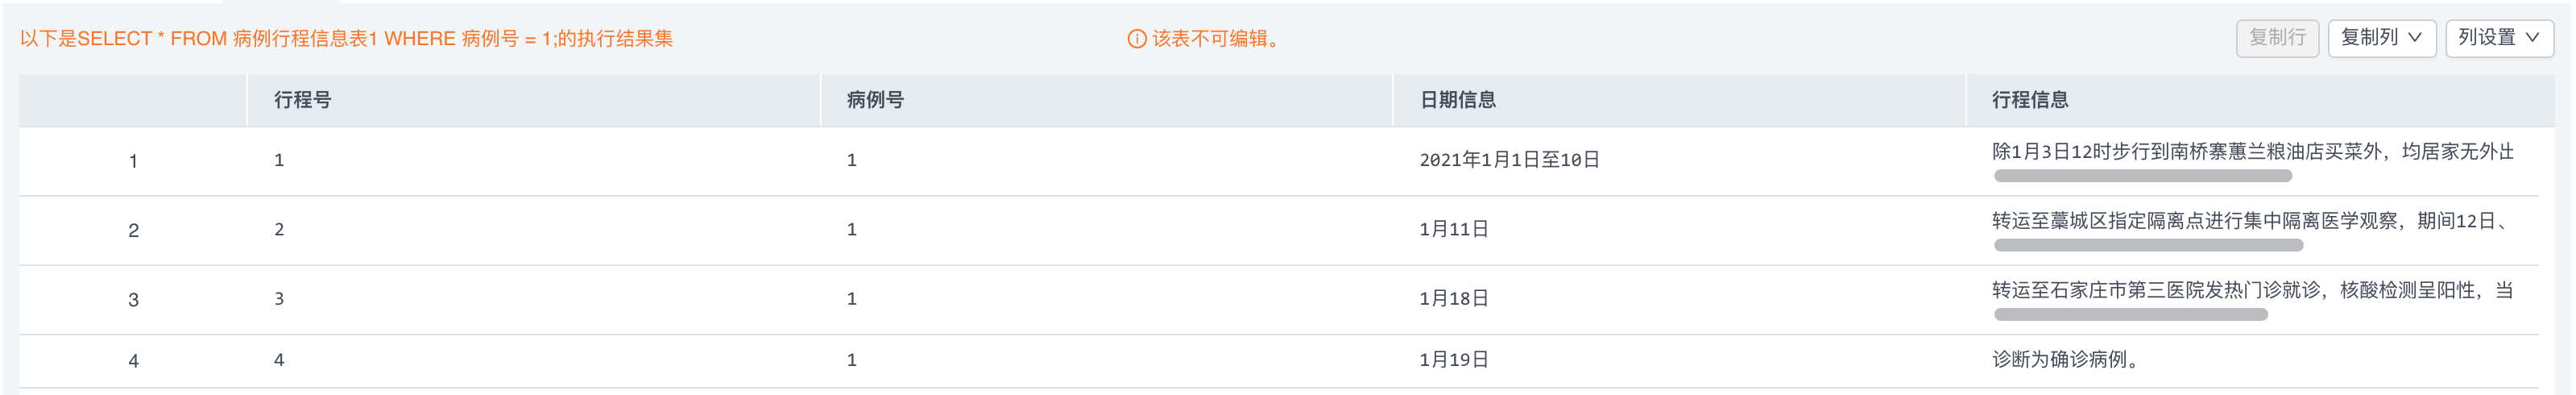
\includegraphics[width=\textwidth]{./images/res37.png}
    \caption{\label{fig:res37}}
\end{figure}

输入以下SQL语句测试:
\begin{code}
\begin{minted}{sql}
DELETE FROM 病例基本信息表1 WHERE 病例号 = 1;
\end{minted}
\end{code}

结果如\figref{fig:res38}。
\begin{figure}[!htb]
    \centering
    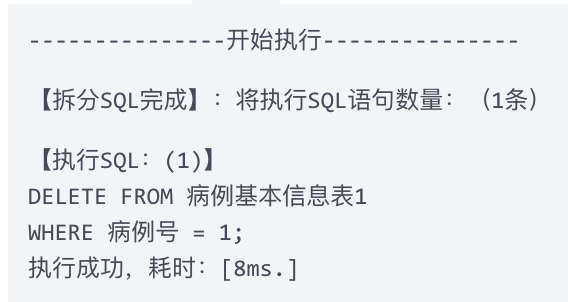
\includegraphics[width=0.4\textwidth]{./images/res38.png}
    \caption{\label{fig:res38}}
\end{figure}

再次查看病例基本信息表和病例行程信息表中病例号为1的患者的信息,如\figref{fig:res39}和\figref{fig:res40}。
\begin{figure}[!htb]
    \centering
    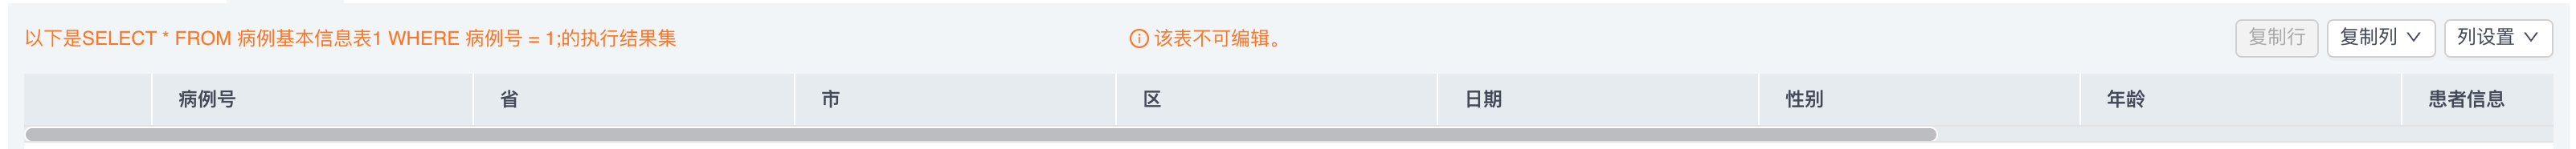
\includegraphics[width=\textwidth]{./images/res39.png}
    \caption{\label{fig:res39}}
\end{figure}
\begin{figure}[!htb]
    \centering
    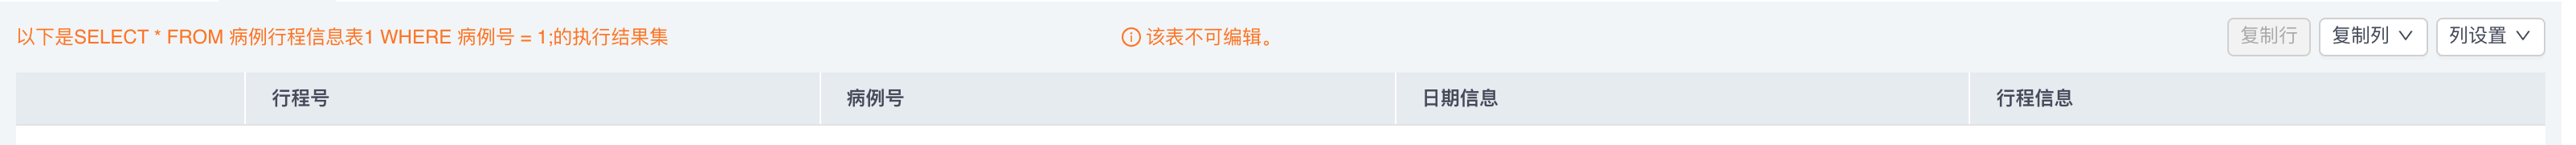
\includegraphics[width=\textwidth]{./images/res40.png}
    \caption{\label{fig:res40}}
\end{figure}

发现两个表中该患者的信息都已经删除。

创建UPDATE触发器,禁止修改全国各省累计数据统计表中的累计确诊、累计治愈和累计死亡数据。

创建函数check\_on\_update,如\figref{fig:res41}。
\begin{figure}[!htb]
    \centering
    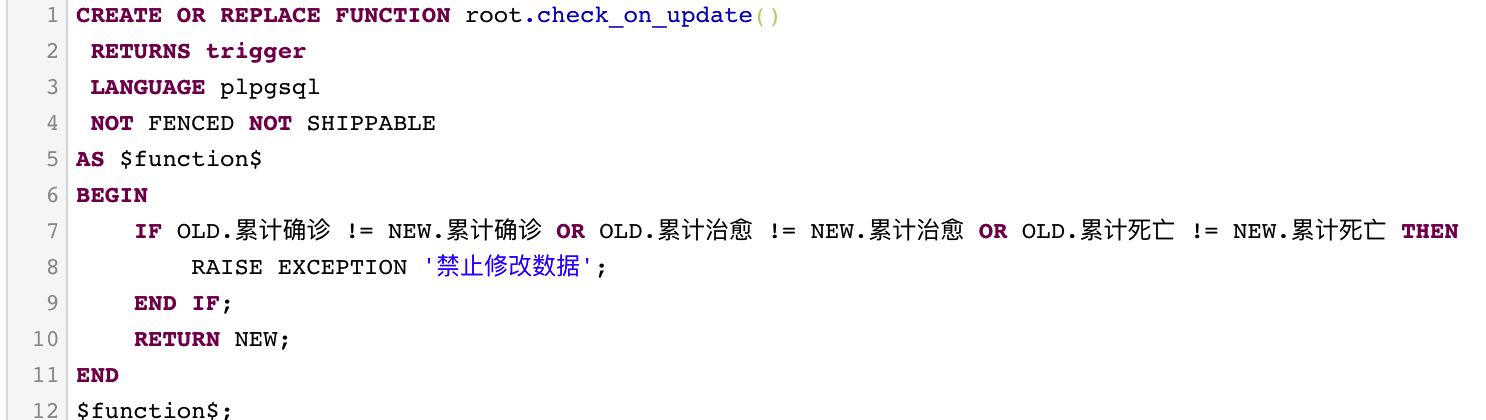
\includegraphics[width=\textwidth]{./images/res41.png}
    \caption{\label{fig:res41}}
\end{figure}

创建触发器,输入以下SQL语句:
\begin{code}
\begin{minted}{sql}
CREATE TRIGGER trigger_update BEFORE UPDATE ON 全国各省累计数据统计表 FOR EACH ROW EXECUTE PROCEDURE check_on_update();
\end{minted}
\end{code}

输入以下SQL语句测试:
\begin{code}
\begin{minted}{sql}
UPDATE 全国各省累计数据统计表 
SET 累计确诊 = 1
WHERE 日期 = '2020-12-31';
\end{minted}
\end{code}

结果如\figref{fig:res42}。
\begin{figure}[!htb]
    \centering
    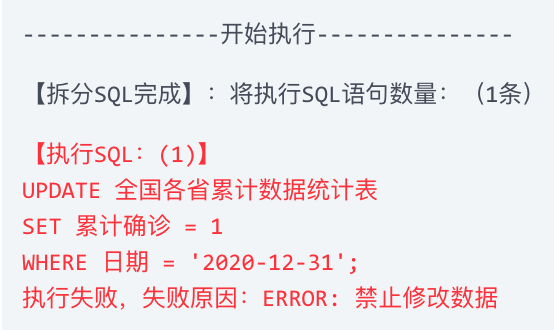
\includegraphics[width=0.4\textwidth]{./images/res42.png}
    \caption{\label{fig:res42}}
\end{figure}

\subsection{管理触发器}

删除INSERT触发器、DELETE触发器、UPDATE触发器,输入以下SQL语句:
\begin{code}
\begin{minted}{sql}
DROP TRIGGER trigger_insert ON 美国各州县确诊与死亡数统计表;
DROP TRIGGER trigger_delete ON 病例基本信息表1;
DROP TRIGGER trigger_update ON 全国各省累计数据统计表;
\end{minted}
\end{code}

结果如\figref{fig:res43}。
\begin{figure}[!htb]
    \centering
    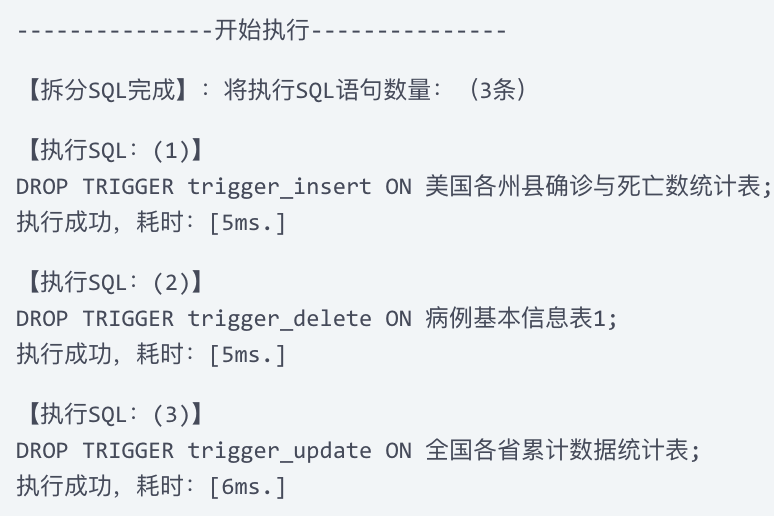
\includegraphics[width=0.4\textwidth]{./images/res43.png}
    \caption{\label{fig:res43}}
\end{figure}

\subsection{事务级全局临时表}

创建临时表t\_test2,输入以下SQL语句:
\begin{code}
\begin{minted}{sql}
CREATE GLOBAL TEMPORARY TABLE t_test2(
    id integer,
    lbl text
) ON COMMIT DELETE ROWS;
\end{minted}
\end{code}

结果如\figref{fig:res44}。
\begin{figure}[!htb]
    \centering
    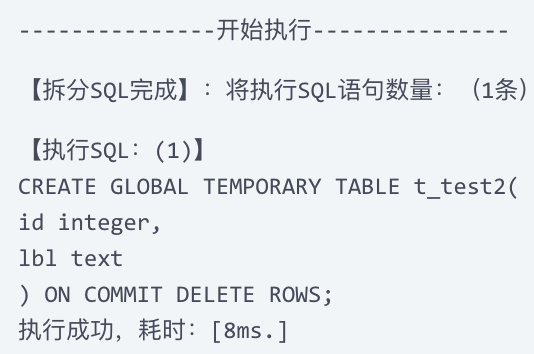
\includegraphics[width=0.4\textwidth]{./images/res44.png}
    \caption{\label{fig:res44}}
\end{figure}

首先,用begin开始一个事务,其次,向表中插入数据,最后,对表进行查询。可以查出相应数据,输入以下SQL语句:
\begin{code}
\begin{minted}{sql}
BEGIN;
INSERT INTO t_test2 VALUES(1,'data1');
SELECT * FROM t_test2;
\end{minted}
\end{code}

结果如\figref{fig:res45}。
\begin{figure}[!htb]
    \centering
    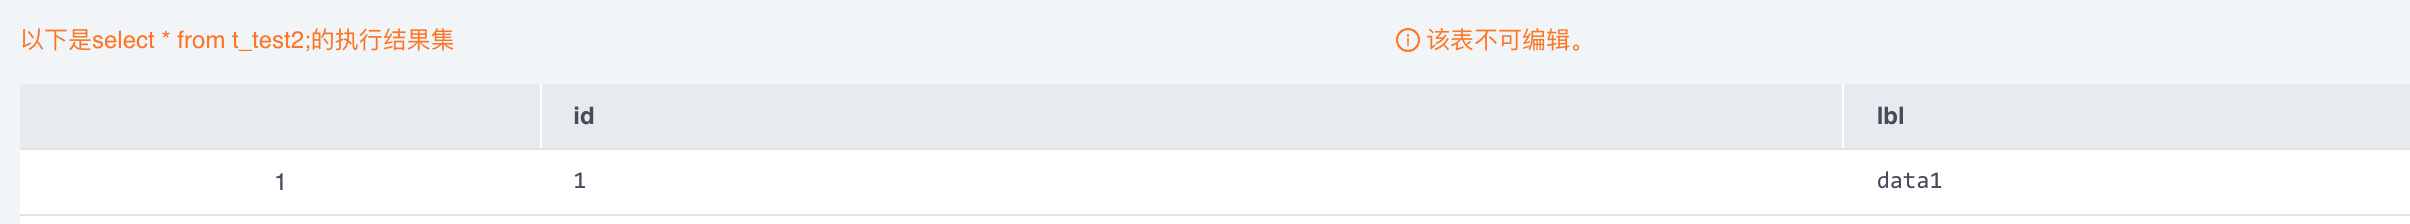
\includegraphics[width=\textwidth]{./images/res45.png}
    \caption{\label{fig:res45}}
\end{figure}

先用commit提交来结束事务,此时再对表进行查询,可以发现已经查询不出数据了,输入以下SQL语句:
\begin{code}
\begin{minted}{sql}
COMMIT;
SELECT * FROM t_test2;
\end{minted}
\end{code}

结果如\figref{fig:res46}。
\begin{figure}[!htb]
    \centering
    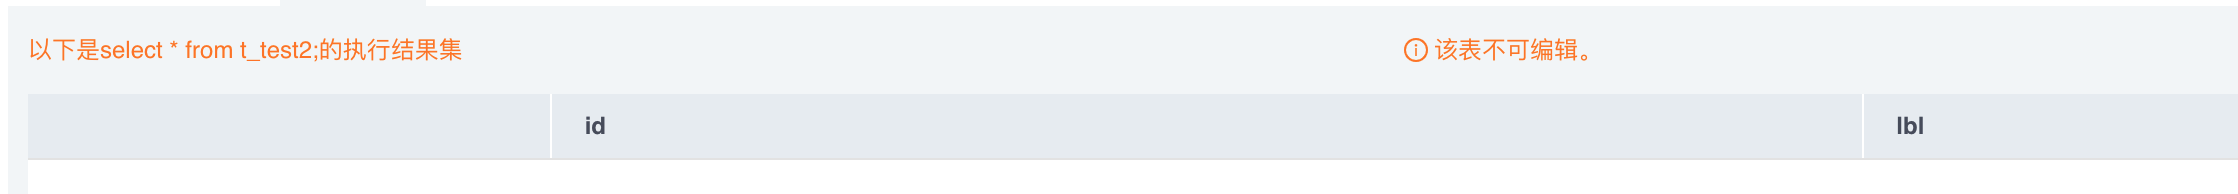
\includegraphics[width=\textwidth]{./images/res46.png}
    \caption{\label{fig:res46}}
\end{figure}

删除临时表,输入以下SQL语句:
\begin{code}
\begin{minted}{sql}
drop table t_test2;
\end{minted}
\end{code}

结果如\figref{fig:res47}。
\begin{figure}[!htb]
    \centering
    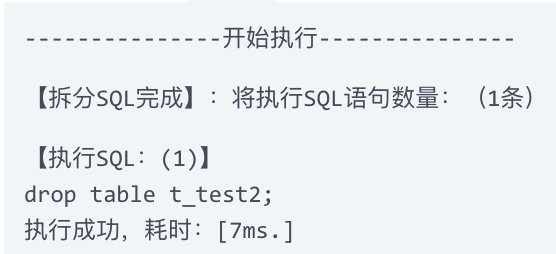
\includegraphics[width=0.4\textwidth]{./images/res47.png}
    \caption{\label{fig:res47}}
\end{figure}

\section{实验总结}

实验中,我参考PostgreSQL的语法说明和教材上的内容编写存储过程和触发器的SQL语句,使我对SQL语法的熟悉程度大大增加,同时增强了我的英文文献阅读能力。

本次实验使我对触发器的理解更加深刻,同时巩固了课堂上所学的有关触发器的知识。

\part{实验七}

\section{概述}

\subsection{实验目的}

\begin{enumerate}
    \item 华为的GaussDB(for openGauss)支持基于C、Java等应用程序的开发。了解它相关的系统结构和相关概念,有助于更好地开发和使用GaussDB(for openGauss)数据库。
    \item 通过实验了解通用数据库应用编程接口ODBC/JDBC的基本原理和实现机制,熟悉连接ODBC/JDBC接口的语法和使用方法。
    \item 熟练GaussDB(for openGauss)的各种连接方式与常用工具的使用。
    \item 利用C语言(或其它支持ODBC/JDBC接口的高级程序设计语言)编程实现简单的数据库应用程序,掌握基于ODBC的数据库访问基本原理和方法。
\end{enumerate}

\subsection{实验平台及环境}

\begin{itemize}
    \item GaussDB(for openGauss) 8 核 | 64 GB
    \item GaussDB(for openGauss) 2020主备版
    \item Windows 10 Pro 21H1
    \item MinGW-w64 8.1.0
\end{itemize}

\subsection{实验内容}

\begin{enumerate}
    \item 本实验内容通过使用ODBC/JDBC等驱动开发应用程序。
    \item 连接语句访问数据库接口,实现对数据库中的数据进行操作(包括增、删、改、查等);
    \item 要求能够通过编写程序访问到华为数据库,该实验重点在于ODBC/JDBC数据源配置和高级语言(C/C++/Java/Python)的使用。
\end{enumerate}

\section{实验步骤}

\subsection{配置数据源}

下载\mintinline{text}{GaussDB-Kernel-V500R001C10-Windows-Odbc.tar.gz}并解压,点击\mintinline{text}{psqlodbc_x64.msi}进行安装。

进入\mintinline{text}{C:\Windows\System32\odbcad32.exe},选择用户DSN->添加->PostgreSQL Unicode,输入用户名和密码,点击测试,如\figref{fig:source}所示。测试成功后保存并退出。

\begin{figure}[!htb]
    \centering
    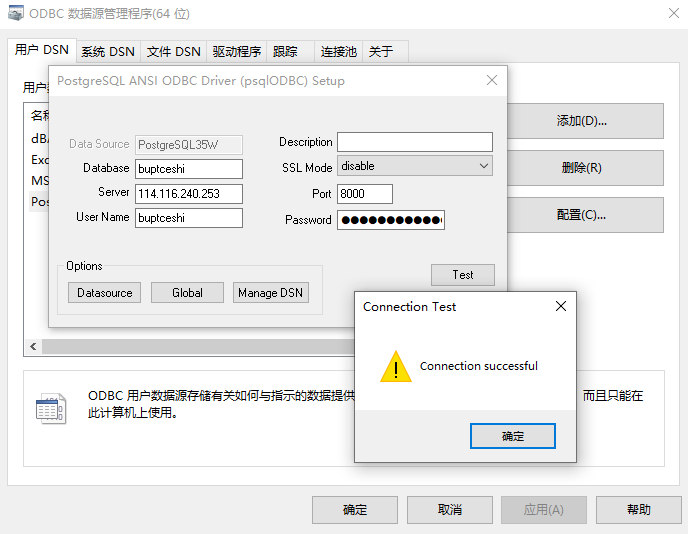
\includegraphics[width=0.6\textwidth]{./images/source.png}
    \caption{配置数据源\label{fig:source}}
\end{figure}

\subsection{编写程序}

\begin{code}
\begin{minted}{C}
#include <stdlib.h>
#include <stdio.h>
#include <wchar.h>
#ifdef WIN32
#include <windows.h>
#endif
#include <sqlext.h>
#include <locale.h>

SQLHENV V_OD_Env; // 环境句柄
SQLHSTMT V_OD_hstmt; // 句柄
SQLHDBC V_OD_hdbc; // 连接属性
SQLINTEGER V_OD_erg, V_OD_err; // 存放返回值
SQL_DATE_STRUCT date;
SQLWCHAR prov[50];
SQLINTEGER defi, cure, death;
SQLLEN cb_date, cb_prov, cb_defi, cb_cure, cb_death;
SQLLEN res_cnt;
char query[200]; // 存放查询语句

int main(int argc, char *argv)
{
    // 区域设置,用于处理中文
    setlocale(LC_ALL, "");
    // 申请环境句柄
    V_OD_erg = SQLAllocHandle(SQL_HANDLE_ENV, SQL_NULL_HANDLE, &V_OD_Env);
    if ((V_OD_erg != SQL_SUCCESS) && (V_OD_erg != SQL_SUCCESS_WITH_INFO))
    {
        printf("Error AllocHandle\n");
        exit(0);
    }
    // 设置环境属性
    SQLSetEnvAttr(V_OD_Env, SQL_ATTR_ODBC_VERSION, (void *)SQL_OV_ODBC3, 0);
    // 申请连接句柄
    V_OD_erg = SQLAllocHandle(SQL_HANDLE_DBC, V_OD_Env, &V_OD_hdbc);
    if ((V_OD_erg != SQL_SUCCESS) && (V_OD_erg != SQL_SUCCESS_WITH_INFO))
    {
        SQLFreeHandle(SQL_HANDLE_ENV, V_OD_Env);
        exit(0);
    }
    // 设置连接属性
    SQLSetConnectAttr(V_OD_hdbc, SQL_ATTR_AUTOCOMMIT, (SQLPOINTER)SQL_AUTOCOMMIT_ON, 0);
    // 连接数据源
    V_OD_erg = SQLConnect(V_OD_hdbc, (SQLCHAR *)"PostgreSQL35W", SQL_NTS, (SQLCHAR *)"buptceshi", SQL_NTS, (SQLCHAR *)"bupt20211201@", SQL_NTS);
    if ((V_OD_erg != SQL_SUCCESS) && (V_OD_erg != SQL_SUCCESS_WITH_INFO))
    {
        printf("Error SQLConnect %d\n", V_OD_erg);
        SQLFreeHandle(SQL_HANDLE_ENV, V_OD_Env);
        exit(0);
    }
    printf("Connected!\n");
    // 设置语句属性
    SQLSetStmtAttr(V_OD_hstmt, SQL_ATTR_QUERY_TIMEOUT, (SQLPOINTER *)3, 0);
    // 申请语句句柄
    SQLAllocHandle(SQL_HANDLE_STMT, V_OD_hdbc, &V_OD_hstmt);

    // 将长字符的字符串转为多字节的字符串
    wcstombs_s(NULL, query, 200, L"SELECT * FROM root.全国各省累计数据统计表 WHERE 日期 = '2020-12-8'", _TRUNCATE);
    // 执行查询
    SQLExecDirect(V_OD_hstmt, query, SQL_NTS);
    // 绑定结果集
    SQLBindCol(V_OD_hstmt, 1, SQL_C_TYPE_DATE, (SQLPOINTER)&date, 50, &cb_date);
    SQLBindCol(V_OD_hstmt, 2, SQL_C_WCHAR, (SQLPOINTER)prov, 50, &cb_prov);
    SQLBindCol(V_OD_hstmt, 3, SQL_C_SLONG, (SQLPOINTER)&defi, 50, &cb_defi);
    SQLBindCol(V_OD_hstmt, 4, SQL_C_SLONG, (SQLPOINTER)&cure, 50, &cb_cure);
    SQLBindCol(V_OD_hstmt, 5, SQL_C_SLONG, (SQLPOINTER)&death, 50, &cb_death);
    // 取一条数据
    V_OD_erg = SQLFetch(V_OD_hstmt);
    while (V_OD_erg != SQL_NO_DATA)
    {
        printf("%S: %d-%d-%d %S: %S %S: %d %S: %d %S: %d\n", L"日期", date.year, date.month, date.day, L"省", prov, L"累计确诊", defi, L"累计治愈", cure, L"累计死亡", death);
        // 取下一条数据
        V_OD_erg = SQLFetch(V_OD_hstmt);
    }
    printf("Query Done!\n\n");
    // 释放游标
    SQLCloseCursor(V_OD_hstmt);

    wcstombs_s(NULL, query, 200, L"INSERT INTO root.全国各省累计数据统计表 values(?,?,?,?,?)", _TRUNCATE);
    // 准备执行
    SQLPrepare(V_OD_hstmt, query, SQL_NTS);
    // 准备参数
    date.year = 2021;
    date.month = 10;
    date.day = 8;
    wcscpy(prov, L"吉林省");
    defi = 578;
    cure = 571;
    death = 3;
    // 绑定参数
    SQLBindParameter(V_OD_hstmt, 1, SQL_PARAM_INPUT, SQL_C_TYPE_DATE, SQL_TYPE_DATE, sizeof(date), 0, (SQLPOINTER)&date, 0, &cb_date);
    SQLBindParameter(V_OD_hstmt, 2, SQL_PARAM_INPUT, SQL_C_WCHAR, SQL_WCHAR, 50, 0, (SQLPOINTER)prov, 0, &cb_prov);
    SQLBindParameter(V_OD_hstmt, 3, SQL_PARAM_INPUT, SQL_C_SLONG, SQL_INTEGER, 0, 0, (SQLPOINTER)&defi, 0, &cb_defi);
    SQLBindParameter(V_OD_hstmt, 4, SQL_PARAM_INPUT, SQL_C_SLONG, SQL_INTEGER, 0, 0, (SQLPOINTER)&cure, 0, &cb_cure);
    SQLBindParameter(V_OD_hstmt, 5, SQL_PARAM_INPUT, SQL_C_SLONG, SQL_INTEGER, 0, 0, (SQLPOINTER)&death, 0, &cb_death);
    // 执行
    SQLExecute(V_OD_hstmt);
    // 提取行计数
    SQLRowCount(V_OD_hstmt, &res_cnt);
    printf("Inserted %d row.\n\n", res_cnt);

    wcstombs_s(NULL, query, 200, L"SELECT * FROM root.全国各省累计数据统计表 WHERE 日期 = '2021-10-8'", _TRUNCATE);
    SQLExecDirect(V_OD_hstmt, query, SQL_NTS);
    V_OD_erg = SQLFetch(V_OD_hstmt);
    while (V_OD_erg != SQL_NO_DATA)
    {
        // 通过SQLGetData取数据
        SQLGetData(V_OD_hstmt, 1, SQL_C_TYPE_DATE, (SQLPOINTER)&date, 50, &cb_date);
        SQLGetData(V_OD_hstmt, 2, SQL_C_WCHAR, (SQLPOINTER)prov, 50, &cb_prov);
        SQLGetData(V_OD_hstmt, 3, SQL_C_SLONG, (SQLPOINTER)&defi, 50, &cb_defi);
        SQLGetData(V_OD_hstmt, 4, SQL_C_SLONG, (SQLPOINTER)&cure, 50, &cb_cure);
        SQLGetData(V_OD_hstmt, 5, SQL_C_SLONG, (SQLPOINTER)&death, 50, &cb_death);
        printf("%S: %d-%d-%d %S: %S %S: %d %S: %d %S: %d\n", L"日期", date.year, date.month, date.day, L"省", prov, L"累计确诊", defi, L"累计治愈", cure, L"累计死亡", death);
        V_OD_erg = SQLFetch(V_OD_hstmt);
    }
    printf("Query Done!\n\n");
    SQLCloseCursor(V_OD_hstmt);

    wcstombs_s(NULL, query, 200, L"UPDATE root.全国各省累计数据统计表 SET 累计确诊 = 0 WHERE 日期 = '2021-10-8'", _TRUNCATE);
    SQLExecDirect(V_OD_hstmt, query, SQL_NTS);
    SQLRowCount(V_OD_hstmt, &res_cnt);
    printf("Updated %d row.\n\n", res_cnt);

    wcstombs_s(NULL, query, 200, L"SELECT * FROM root.全国各省累计数据统计表 WHERE 日期 = '2021-10-8'", _TRUNCATE);
    SQLExecDirect(V_OD_hstmt, query, SQL_NTS);
    V_OD_erg = SQLFetch(V_OD_hstmt);
    while (V_OD_erg != SQL_NO_DATA)
    {
        SQLGetData(V_OD_hstmt, 1, SQL_C_TYPE_DATE, (SQLPOINTER)&date, 50, &cb_date);
        SQLGetData(V_OD_hstmt, 2, SQL_C_WCHAR, (SQLPOINTER)prov, 50, &cb_prov);
        SQLGetData(V_OD_hstmt, 3, SQL_C_SLONG, (SQLPOINTER)&defi, 50, &cb_defi);
        SQLGetData(V_OD_hstmt, 4, SQL_C_SLONG, (SQLPOINTER)&cure, 50, &cb_cure);
        SQLGetData(V_OD_hstmt, 5, SQL_C_SLONG, (SQLPOINTER)&death, 50, &cb_death);
        printf("%S: %d-%d-%d %S: %S %S: %d %S: %d %S: %d\n", L"日期", date.year, date.month, date.day, L"省", prov, L"累计确诊", defi, L"累计治愈", cure, L"累计死亡", death);
        V_OD_erg = SQLFetch(V_OD_hstmt);
    }
    printf("Query Done!\n\n");
    SQLCloseCursor(V_OD_hstmt);

    wcstombs_s(NULL, query, 200, L"DELETE FROM root.全国各省累计数据统计表 WHERE 日期 = '2021-10-8'", _TRUNCATE);
    SQLExecDirect(V_OD_hstmt, query, SQL_NTS);
    SQLRowCount(V_OD_hstmt, &res_cnt);
    printf("Deleted %d row.\n\n", res_cnt);

    wcstombs_s(NULL, query, 200, L"SELECT * FROM root.全国各省累计数据统计表 WHERE 日期 = '2021-10-8'", _TRUNCATE);
    SQLExecDirect(V_OD_hstmt, query, SQL_NTS);
    V_OD_erg = SQLFetch(V_OD_hstmt);
    while (V_OD_erg != SQL_NO_DATA)
    {
        SQLGetData(V_OD_hstmt, 1, SQL_C_TYPE_DATE, (SQLPOINTER)&date, 50, &cb_date);
        SQLGetData(V_OD_hstmt, 2, SQL_C_WCHAR, (SQLPOINTER)prov, 50, &cb_prov);
        SQLGetData(V_OD_hstmt, 3, SQL_C_SLONG, (SQLPOINTER)&defi, 50, &cb_defi);
        SQLGetData(V_OD_hstmt, 4, SQL_C_SLONG, (SQLPOINTER)&cure, 50, &cb_cure);
        SQLGetData(V_OD_hstmt, 5, SQL_C_SLONG, (SQLPOINTER)&death, 50, &cb_death);
        printf("%S: %d-%d-%d %S: %S %S: %d %S: %d %S: %d\n", L"日期", date.year, date.month, date.day, L"省", prov, L"累计确诊", defi, L"累计治愈", cure, L"累计死亡", death);
        V_OD_erg = SQLFetch(V_OD_hstmt);
    }
    printf("Query Done!\n\n");
    SQLCloseCursor(V_OD_hstmt);

    // 断开数据源连接并释放句柄
    SQLFreeHandle(SQL_HANDLE_STMT, V_OD_hstmt);
    SQLDisconnect(V_OD_hdbc);
    SQLFreeHandle(SQL_HANDLE_DBC, V_OD_hdbc);
    SQLFreeHandle(SQL_HANDLE_ENV, V_OD_Env);
    return 0;
}
\end{minted}
\end{code}

程序首先查询国内2021年12月8日的所有确诊信息,之后向表中插入一条2021年10月8日吉林省的数据,紧接着查询该日的所有数据,之后将该行数据中的确诊数改为0,再查询一次,最后删除该行数据,再查询一次。

注:\mintinline{text}{SQLAllocEnv}、\mintinline{text}{SQLAllocConnect}等函数在ODBC 3.0版本中已弃用,用相同功能的函数替代。

\subsection{编译}

\begin{code}
\begin{minted}{shell}
gcc -o A A.c -lodbc32
\end{minted}
\end{code}

\subsection{运行}

运行截图如\figref{fig:running}。

\begin{figure}[!htb]
    \centering
    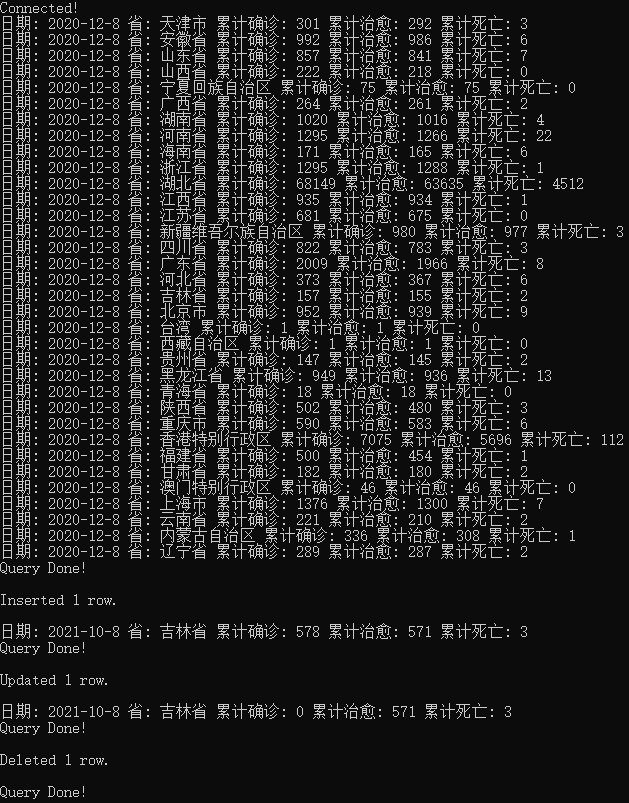
\includegraphics[width=0.7\textwidth]{./images/running.png}
    \caption{运行截图\label{fig:running}}
\end{figure}

\section{实验总结}

在配置数据源环节,按照华为云的文档完成,没有产生问题,但是测试华为云的样例时,发现没有建表权限,并且无论如何替换表名都查询不到表,通过\mintinline{text}{SQLGetDiagField}诊断函数得到报错42501和42P01。

之后尝试使用\mintinline{sql}{SELECT * FROM pg_catalog.pg_tables}语句查看所有表的属性,发现打印出乱码,于是加上了长字符(\mintinline{text}{wchar_t})的字符串和地区设置,正确打印了结果。

发现长字符的查询语句无法直接执行,于是使用\mintinline{text}{wcstombs_s}函数转为多字节的字符串再执行,终于查询出了结果。

在查询完成后,下一条查询报HY010错误,查看文档发现需要通过\mintinline{text}{SQLCloseCursor}释放游标。

\subsection{数据库驱动的概念}

数据库驱动是应用程序和数据库存储之间的一种接口,如\figref{fig:driver}所示,数据库厂商为了某一种开发语言环境(比如Java,C)能够实现数据库调用而开发的类似翻译员功能的程序,将复杂的数据库操作与通信抽象成为了当前开发语言的访问接口。

\begin{figure}[!htb]
    \centering
    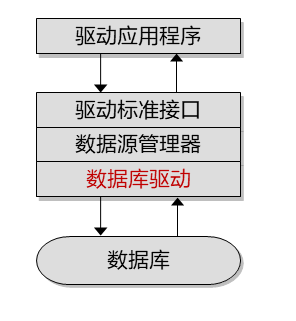
\includegraphics[width=0.3\textwidth]{./images/driver.png}
    \caption{数据库驱动\label{fig:driver}}
\end{figure}

\subsection{使用ODBC开发的流程}

\begin{figure}[htbp]
    \centering
    \subfigure[]{
        \begin{minipage}[t]{0.6\linewidth}
            \centering
            \includegraphics[width=\textwidth]{./images/flow.png}
        \end{minipage}
    }
    \subfigure[]{
        \begin{minipage}[t]{0.2\linewidth}
            \centering
            \includegraphics[width=\textwidth]{./Images/flow_huawei.png}
        \end{minipage}
    }
    \caption{使用ODBC开发的流程\label{fig:flow}}
\end{figure}

使用ODBC开发的流程如\figref{fig:flow}所示。

\begin{enumerate}
    \item 任何应用程序中的第一步是连接到数据源。连接到数据源的第一步是加载驱动程序管理器,然后使用\mintinline{text}{SQLAllocHandle}分配环境句柄。然后,应用程序使用\mintinline{text}{SQL_ATTR_APP_ODBC_VER}属性调用\mintinline{text}{SQLSetEnvAttr}来注册它所遵循的ODBC版本。接下来,应用程序使用\mintinline{text}{SQLAllocHandle}分配连接句柄,然后使用\mintinline{text}{SQLConnect}、\mintinline{text}{SQLDriverConnect}或\mintinline{text}{SQLBrowseConnect}连接到数据源。然后,应用程序设置任何连接属性,例如是否手动提交事务。
    \item 第二步是初始化应用程序。此时,通常使用\mintinline{text}{SQLGetInfo}来发现驱动程序的功能。所有应用程序都需要使用\mintinline{text}{SQLAllocHandle}来分配语句句柄,许多应用程序使用\mintinline{text}{SQLSetStmtAttr}设置语句属性(如游标类型)。
    \item 第三步是生成并执行SQL语句。用于执行此步骤的方法可能会有很大差异。应用程序可能会提示用户输入SQL语句,根据用户输入生成SQL语句,或者使用硬编码的SQL语句。如果SQL语句包含参数,则应用程序会通过对每个参数调用\mintinline{text}{SQLBindParameter},将这些参数绑定到应用程序变量中。生成SQL语句并绑定任何参数后,将通过\mintinline{text}{SQLExecDirect}执行语句。如果语句将多次执行,则可以通过\mintinline{text}{SQLPrepare}准备,并通过\mintinline{text}{SQLExecute}执行。应用程序还可以放弃地执行SQL语句,而调用函数返回包含目录信息的结果集,如可用的列或表。
    \item \begin{itemize}
    \item 如果在步骤3中执行的语句为\mintinline{text}{SELECT}语句或目录函数,应用程序将首先调用\mintinline{text}{SQLNumResultCols}以确定结果集中的列数。如果应用程序已知道结果集列的数目,则不需要执行此步骤,例如,当在垂直或自定义应用程序中对SQL语句进行硬编码时。接下来,应用程序通过\mintinline{text}{SQLDescribeCol}检索每个结果集列的名称、数据类型、精度和小数位数。同样,对于已知道此信息的应用程序(如垂直和自定义应用程序),这并不是必需的。应用程序将此信息传递给\mintinline{text}{SQLBindCol},这会将应用程序变量绑定到结果集中的列。现在,应用程序会调用\mintinline{text}{SQLFetch}来检索第一行数据,并将该行中的数据置于与\mintinline{text}{SQLBindCol}绑定的变量中。如果行中有任何长数据,则它会调用\mintinline{text}{SQLGetData}来检索该数据。应用程序继续调用\mintinline{text}{SQLFetch}和\mintinline{text}{SQLGetData}以检索其他数据。完成数据提取后,它将调用\mintinline{text}{SQLCloseCursor}以关闭游标。现在,应用程序返回到步骤3来执行同一事务中的另一个语句;或转到步骤5以提交或回滚事务。
    \item 如果步骤3中执行的语句是\mintinline{text}{UPDATE}、\mintinline{text}{DELETE}或\mintinline{text}{INSERT}语句,则应用程序使用\mintinline{text}{SQLRowCount}检索受影响的行的计数。应用程序现在返回到步骤3,以在同一事务中执行另一个语句,或继续执行步骤5以提交或回滚事务。
    \end{itemize}
    \item 第五步是调用\mintinline{text}{SQLEndTran}来提交或回滚事务。仅当应用程序将事务提交模式设置为手动提交时,应用程序才会执行此步骤;如果事务提交模式为自动提交(这是默认值),则执行语句时,将自动提交事务。若要在新事务中执行语句,应用程序会返回到步骤3。若要断开与数据源的连接,应用程序将继续执行步骤6。
    \item 最后一步是断开与数据源的连接。首先,应用程序通过调用\mintinline{text}{SQLFreeHandle}释放所有语句句柄。接下来,应用程序与\mintinline{text}{SQLDisconnect}断开与数据源的连接,并通过\mintinline{text}{SQLFreeHandle}释放连接句柄。最后,应用程序通过\mintinline{text}{SQLFreeHandle}释放环境句柄,并卸载驱动程序管理器。
\end{enumerate}

\end{document}